\documentclass[cs4size,a4paper,10pt]{ctexart}   

\linespread{1.5}
\usepackage{geometry}%用于设置上下左右页边距
	\geometry{left=2.5cm,right=2.5cm,top=3.2cm,bottom=2.7cm}
\usepackage{xeCJK,amsmath,paralist,enumerate,booktabs,multirow,graphicx,subfig,setspace,listings,lastpage,hyperref}
\usepackage{amsthm, amssymb, bm, color, framed, graphicx, hyperref, mathrsfs}
\usepackage{mathrsfs}  
	\setlength{\parindent}{2em}
	\lstset{language=Matlab}%
\usepackage{fancyhdr}
\usepackage{graphicx}
\usepackage{subfloat}
\usepackage{listings}
\usepackage{xcolor}
\usepackage{float}
\usepackage{paralist}
\usepackage{setspace}
\usepackage{titlesec}
\usepackage{enumitem}
\usepackage{hyperref}
\usepackage{multirow}
\usepackage{threeparttable}



\hypersetup{
	colorlinks=true,
	linkcolor=black
}

\setenumerate{partopsep=0pt,topsep=0pt}
\setitemize{itemsep=0pt,partopsep=0pt,topsep=0pt}

\titlespacing*{\section}{0pt}{3pt}{3pt}
\titlespacing*{\subsection}{0pt}{2pt}{2pt}
\titlespacing*{\subsubsection}{0pt}{1pt}{1pt}
\titlespacing*{\paragraph}{0pt}{0pt}{0pt}

\ctexset{secnumdepth=4,tocdepth=4}
\setlength{\parindent}{0pt}
\setstretch{1.2}


\setCJKmainfont[BoldFont={FZHei-B01},ItalicFont={FZKai-Z03}]{FZShuSong-Z01} 
\setCJKsansfont[BoldFont={FZHei-B01}]{FZKai-Z03} 
\setCJKmonofont[BoldFont={FZHei-B01}]{FZFangSong-Z02}
\setCJKfamilyfont{zhsong}{FZShuSong-Z01} 
\setCJKfamilyfont{zhhei}{FZHei-B01} 
\setCJKfamilyfont{zhkai}[BoldFont={FZHei-B01}]{FZKai-Z03} 
\setCJKfamilyfont{zhfs}[BoldFont={FZHei-B01}]{FZFangSong-Z02} 
\renewcommand*{\songti}{\CJKfamily{zhsong}} 
\renewcommand*{\heiti}{\CJKfamily{zhhei}} 
\renewcommand*{\kaishu}{\CJKfamily{zhkai}} 
\renewcommand*{\fangsong}{\CJKfamily{zhfs}}


\definecolor{mKeyword}{RGB}{0,0,255}          % bule
\definecolor{mString}{RGB}{160,32,240}        % purple
\definecolor{mComment}{RGB}{34,139,34}        % green
\definecolor{mNumber}{RGB}{128,128,128} 

\lstdefinestyle {njulisting} {
	basewidth = 0.5 em,
	lineskip = 3 pt,
	basicstyle = \small\ttfamily,
	% keywordstyle = \bfseries,
	commentstyle = \itshape\color{gray}, 
	basicstyle=\small\ttfamily,
	keywordstyle={\color{mKeyword}},     % sets color for keywords
	stringstyle={\color{mString}},       % sets color for strings
	commentstyle={\color{mComment}},     % sets color for comments
	numberstyle=\tiny\color{mNumber},
	numbers = left,
	captionpos = t,
	breaklines = true,
	xleftmargin = 2 em,
	xrightmargin = 2 em,
	frame=tlrb,
	tabsize=4
}

\lstset{
style = njulisting, % 调用上述样式 
flexiblecolumns % 允许调整字符宽度
}


%================= 基本格式预置 ===========================
\usepackage{fancyhdr}
\pagestyle{fancy}
\lhead{\textsc{Computer Networking}}
\rhead{第六章\ 应用层}
\cfoot{\thepage}
\renewcommand{\headrulewidth}{0.4pt}
\renewcommand{\theenumi}{(\arabic{enumi})}
\CTEXsetup[format={\bfseries\zihao{-3}}]{section}
\CTEXsetup[format={\bfseries\zihao{4}}]{subsection}
\CTEXsetup[format={\bfseries\zihao{-4}}]{subsubsection}


\renewcommand{\contentsname}{目录}  
\begin{document}

	\begin{center}
		{\huge\textbf{第六章\ 应用层}}
	\end{center}
	%---------目录---------% 
	\pagenumbering{Roman}
	\tableofcontents
	\clearpage

 	%---------正文---------% 
	\pagenumbering{arabic}
	\setcounter{page}{1}
	\setlength{\parskip}{0.65em}


	\begin{figure}[H]
		\centering
		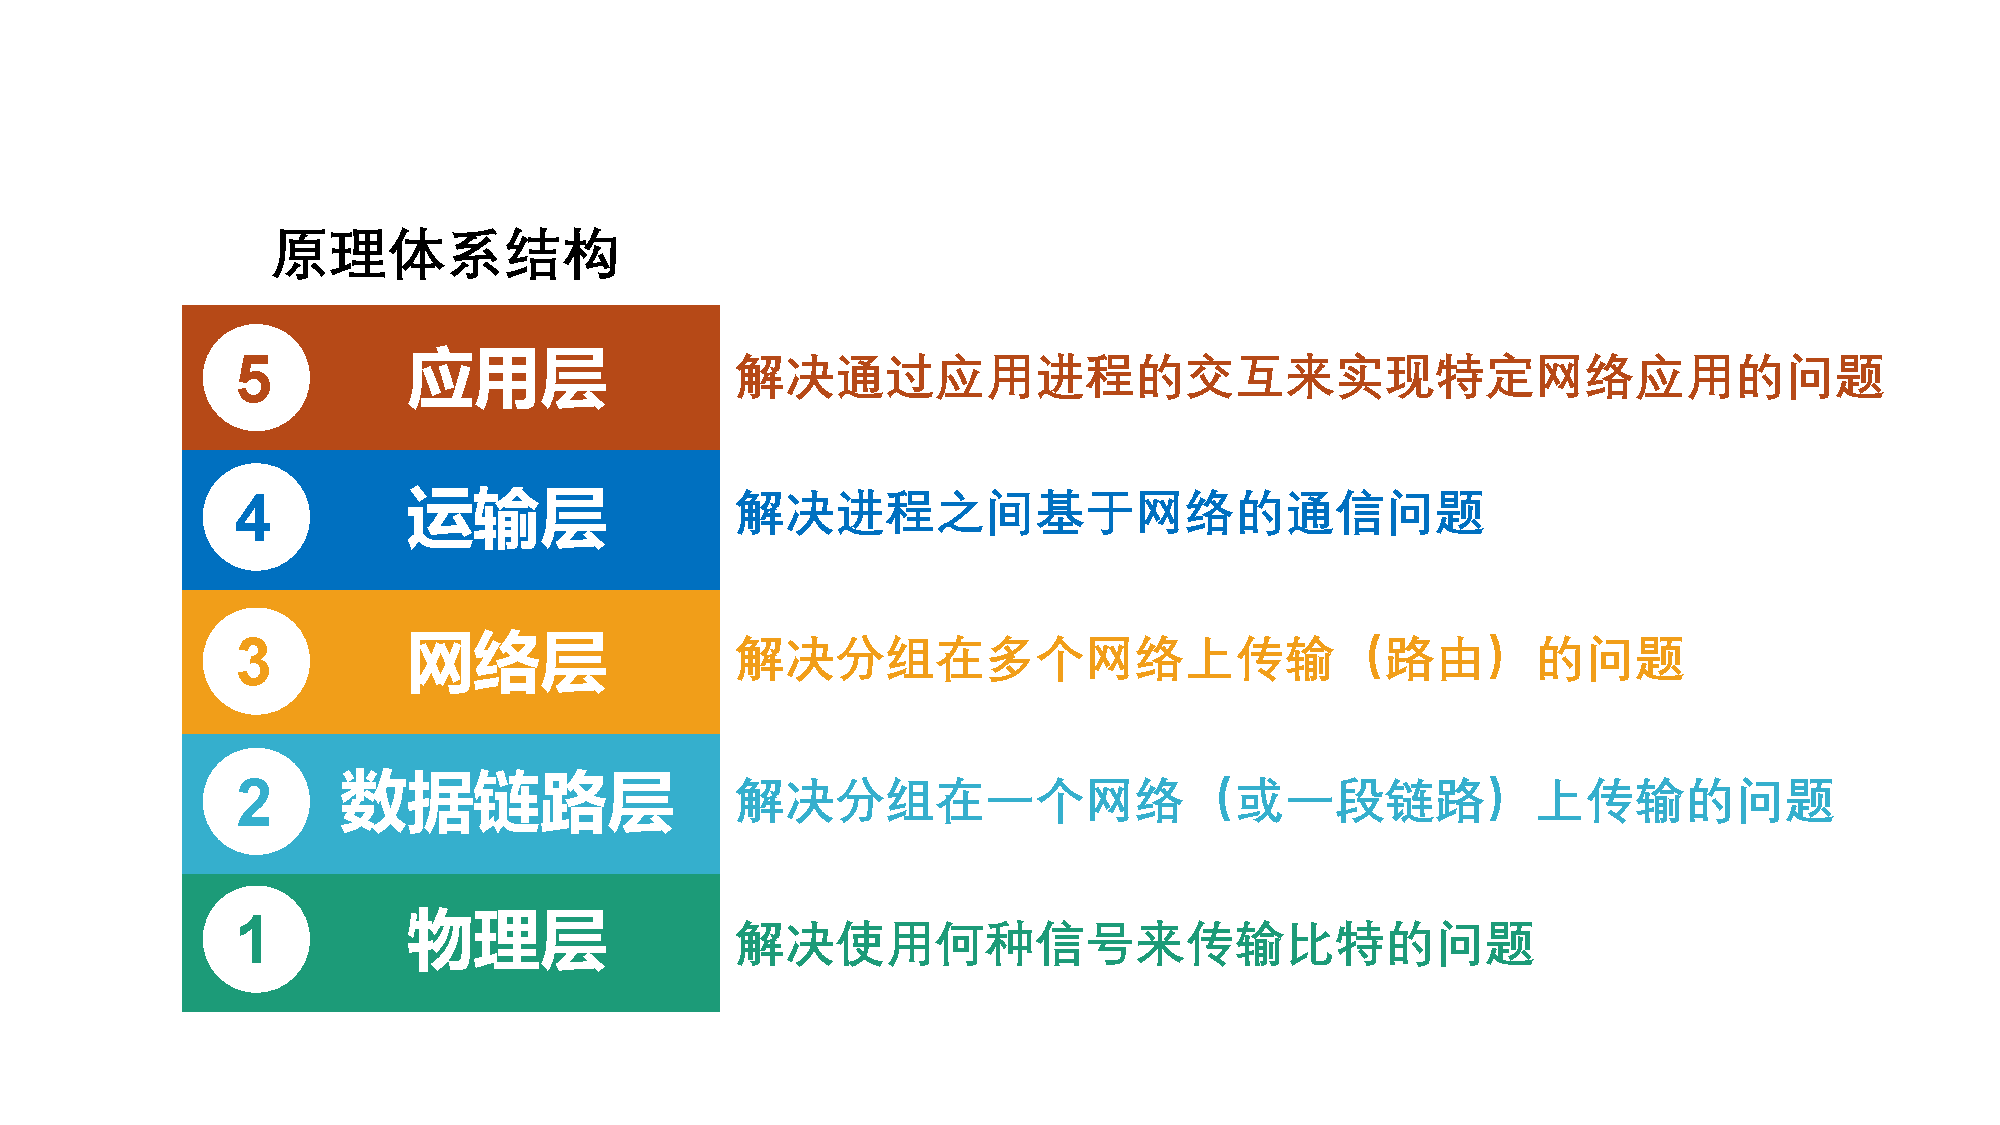
\includegraphics[width=0.8\textwidth]{img/6.0}
	\end{figure}
	
	应用层协议应当定义:
	\begin{itemize}
		\item 应用进程交换的报文类型,如请求报文和响应报文
		\item 各种报文类型的语法,如报文中的各个字段及其详细描述
		\item 字段的语义,即包含在字段中的信息的含义
		\item 进程何时、如何发送报文,以及对报文进行响应的规则
	\end{itemize}

	应用层的许多协议都是基于客户服务器方式。即使是 P2P 对等通信方式,实质上也是一种特殊的客户服务器方式
	\begin{itemize}
		\item 客户和服务器都是指通信中所涉及的两个应用进程
		\item 客户服务器方式所描述的是进程之间服务和被服务的关系
		\item 这里最主要的特征就是:客户是服务请求方,服务器是服务提供方
	\end{itemize}

	\section{域名系统DNS}

	\subsection{域名系统概述}

	\begin{itemize}
		\item 域名系统 DNS(Domain Name System)是互联网使用的命名系统,用来把便于人们使用的机器名字转换为 IP 地址
		\item 互联网的域名系统 DNS 被设计成为一个联机分布式数据库系统,并采用客户服务器方式
		\item DNS 使大多数名字都在本地进行解析(resolve),仅少量解析需要在互联网上通信,因此 DNS 系统的效率很高
		\item 域名到 IP 地址的解析是由分布在互联网上的许多域名服务器程序(可简称为域名服务器)共同完成的
		\item 域名到 IP 地址的解析过程的要点如下:
		\begin{itemize}
			\item 当某一个应用进程需要把主机名解析为 IP 地址时,该应用进程就调用解析程序(resolver),并成为 DNS 的一个客户,把待解析的域名放在 DNS 请求报文中,以 UDP 用户数据报方式发给本地域名服务器(使用 UDP 是为了减少开销)
			\item 本地域名服务器在查找域名后,把对应的 IP 地址放在回答报文中返回。应用进程获得目的主机的 IP 地址后即可进行通信
			\item 若本地域名服务器不能回答该请求,则此域名服务器就暂时成为 DNS 中的另一个客户,并向其他域名服务器发出查询请求。这种过程直至找到能够回答该请求的域名服务器为止
		\end{itemize}
	\end{itemize}

	\subsection{互联网的域名结构}
	\begin{itemize}
		\item 因特网采用层次树状结构的域名结构
		\item 域名的结构由若干个分量组成,各分量之间用“点”隔开,分别代表不同级别的域名
		\begin{center}
			$\cdots$.三级域名.二级域名.顶级域名
		\end{center}
		\begin{itemize}
			\item 每一级的域名都由英文字母和数字组成,不超过 63 个字符,不区分大小写字母
			\item 级别最低的域名写在最左边,而级别最高的顶级域名写在最右边
			\item 完整的域名不超过 255 个字符
		\end{itemize}
		\item 域名系统既不规定一个域名需要包含多少个下级域名,也不规定每一级的域名代表什么意思
		\item 各域名由其上一级的域名管理机构管理,而最高的顶级域名则由因特网名称与数字地址分配机构 ICANN 进行管理
		\item 顶级域名 TLD(top level domain)分为以下三类:
		\begin{itemize}
			\item 国家顶级域名 nTLD:采用 ISO 3166 的规定,如 cn 表示中国,us 表示美国,uk 表示英国等
			\item 通用顶级域名 gTLD:最常见的通用顶级域名有七个,即 com(公司企业)、net(网络服务机构)、org(非营利性组织)、int(国际组织)、edu(美国教育机构)、gov(美国政府部门)、mil(美国军事部门)
			\item 基础结构域名(infrastructure domain):这种域名只有一个,即 arpa,用于反向域名解析,因此又称为反向域名
		\end{itemize}
		\item 在国家顶级域名下注册的二级域名均由该国家自行确定。例如,顶级域名为 jp 的日 本,将其教育和企业机构的二级域名定为 ac 和 co,而不用 edu 和 com
		\item 我国将二级域名划分为以下两类:
		\begin{itemize}
			\item 类别域名:共七个,ac(科研机构)、com(工、商、金融等企业)、edu(教育机构)、gov(政府部门)、net(提供网络服务的机构)、mil(军事机构)和org(非营利性组织)
			\item 行政区域名:共 34 个,适用于我国的各省、自治区和直辖市
		\end{itemize}
	\end{itemize}

	\begin{figure}[H]
		\centering
		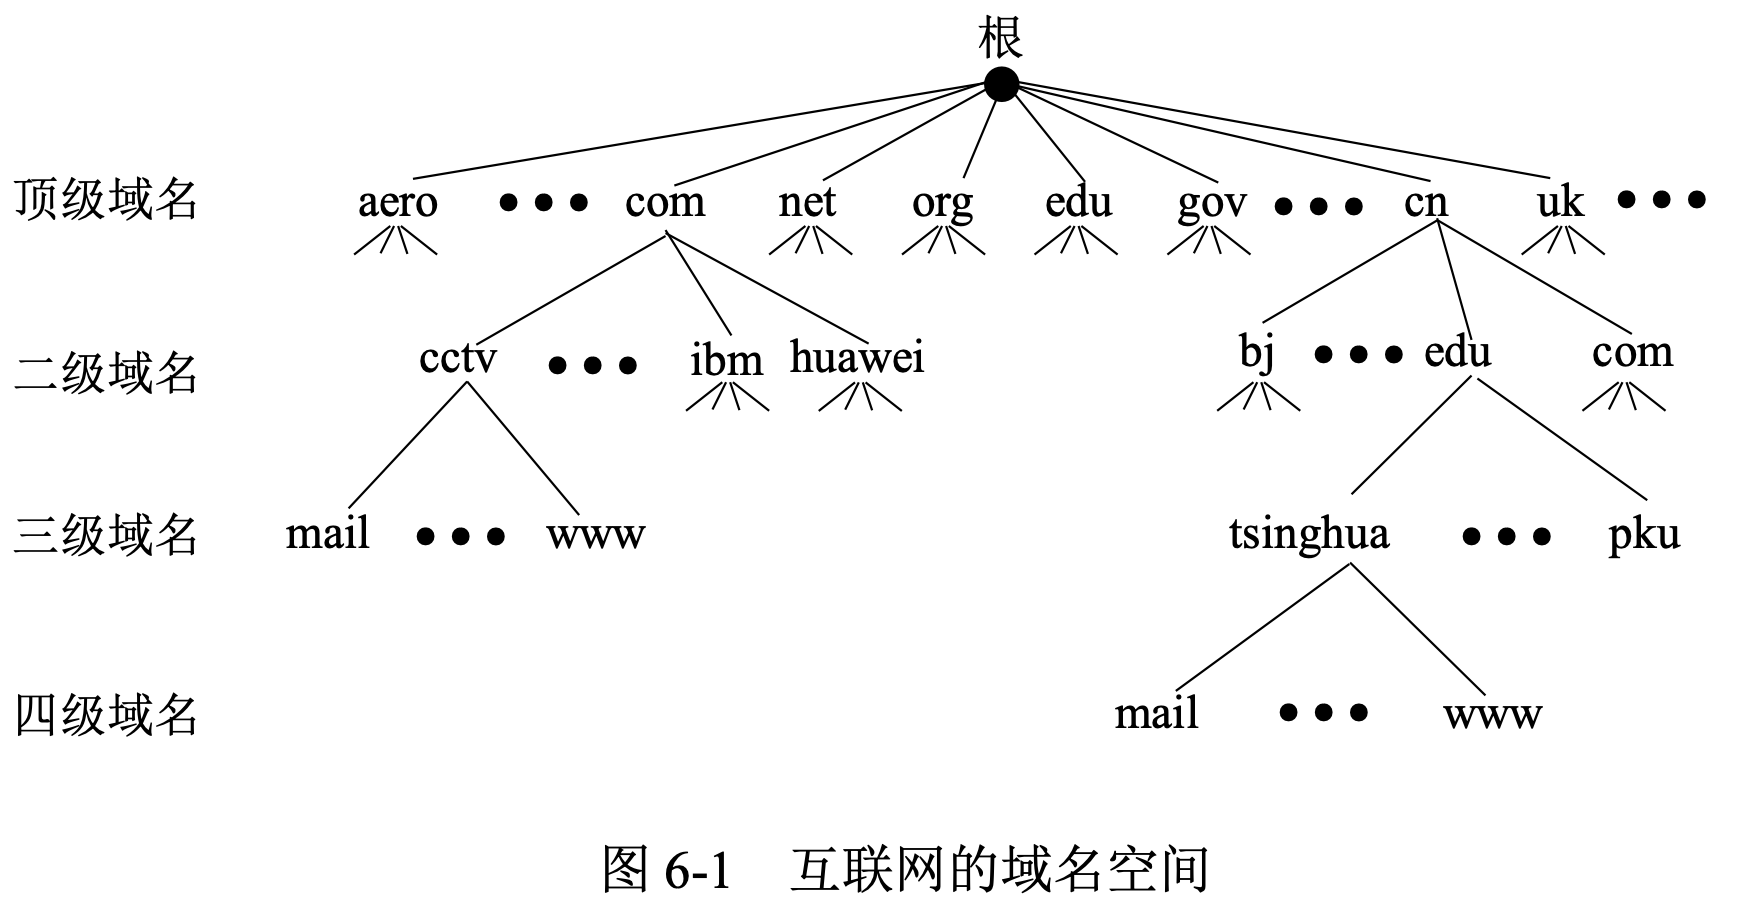
\includegraphics[width=0.7\textwidth]{img/6.1}
	\end{figure}

	\subsection{域名服务器}

	\begin{figure}[H]
		\centering
		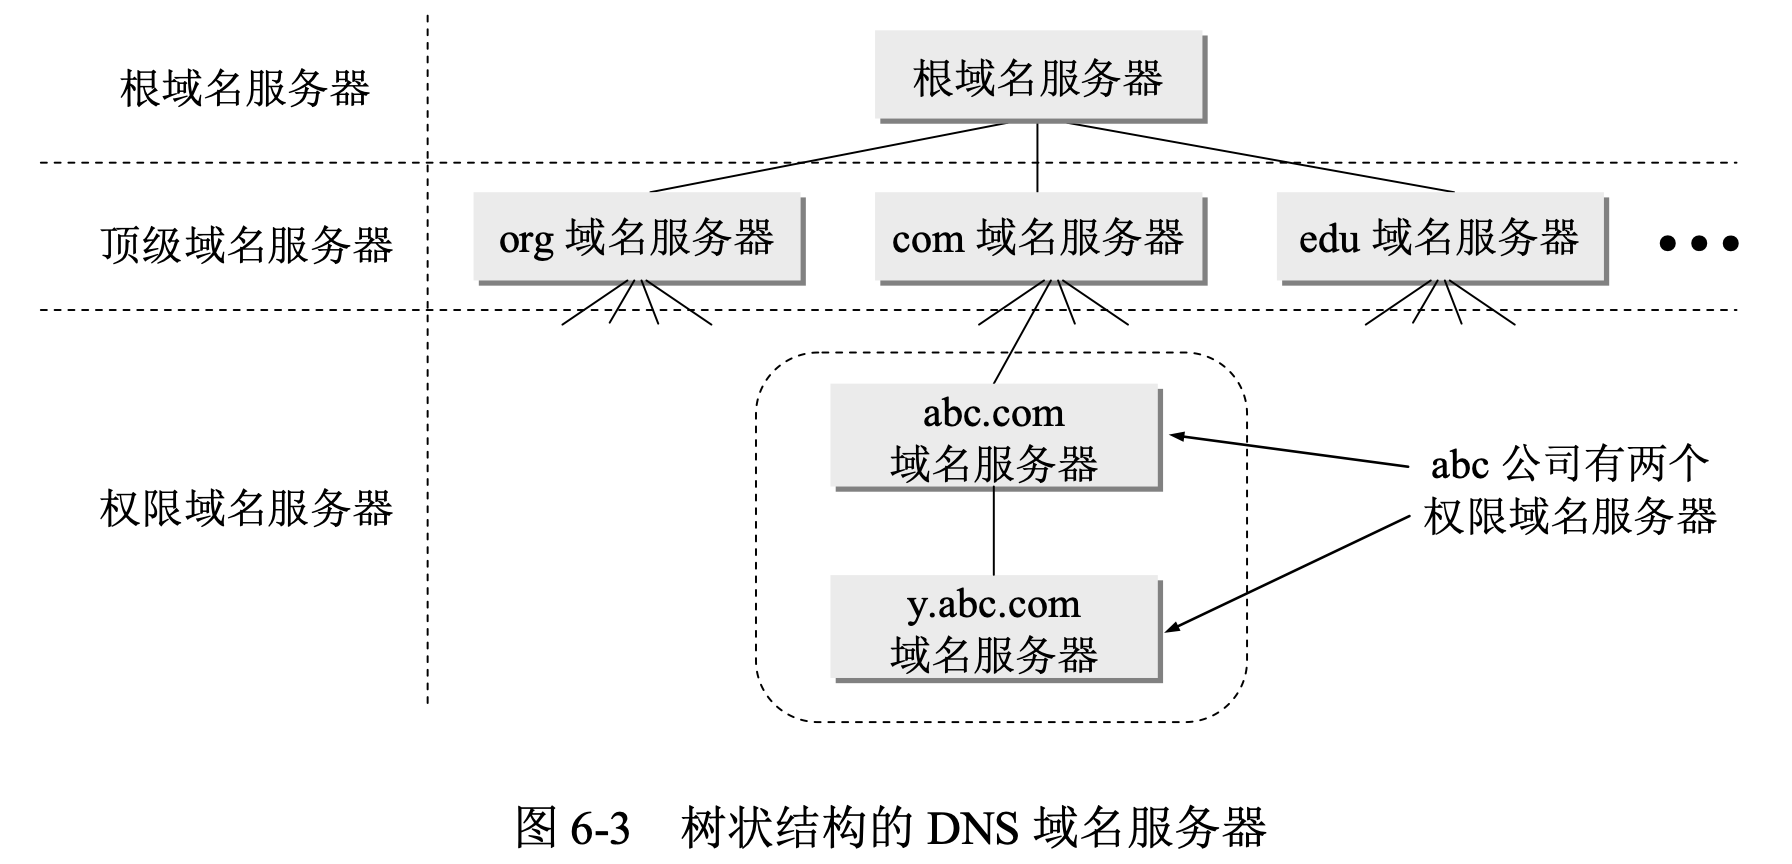
\includegraphics[width=0.7\textwidth]{img/6.3}
	\end{figure}

	\begin{itemize}
		\item 域名和 IP 地址的映射关系必须保存在域名服务器中,供所有其他应用查询。显然不能将所有信息都储存在一台域名服务器中。DNS 使用分布在各地的域名服务器来实现域名到 IP 地址的转换
		\item 域名服务器可以划分为以下四种不同的类型:
		\begin{itemize}
			\item 根域名服务器:根域名服务器是最高层次的域名服务器。每个根域名服务器都知道所有的顶级域名服务器的域名及其 IP 地址。因特网上共有 13 个不同 IP 地址的根域名服务器,尽管我们将这 13 个根域名服务器中的每一个都视为单个的服务器,但“每台服务器”实际上是由许多分布在世界各地的计算机构成的服务器群集。当本地域名服务器向根域名服务器发出查询请求后时,路由器就把查询请求报文转发到离这个 DNS 客户最近到一个根域名服务器。这就加快了 DNS 的查询过程,同时也更合理地利用了因特网的资源。根域名服务器通常并不直接对域名进行解析,而是返回该域名所属顶级域名的顶级域名服务器的 IP 地址
			\item 顶级域名服务器:这些域名服务器负责管理在该顶级域名服务器注册的所有二级域名。当收到 DNS 查询请求时,就给出相应的回答(可能是最后的结果,也可能是下一步应当找的域名服务器的 IP 地址)
			\item 权限域名服务器:这些域名服务器负责管理某个区的域名。每一个主机的域名都必须在某个权限域名服务器处注册登记。因此权限域名服务器知道其所管辖的域名与 IP 地址的映射关系。另外,权限域名服务器还知道其下级域名服务器的地址
			\item 本地域名服务器:本地域名服务器并不属于上述域名服务器层次结构。当一台主机发出 DNS 查询请求时,这个查询请求报文就发送给本地域名服务器。本地域名服务器起着代理的作用,会将该报文转发到上述的域名服务器的等级结构中。每一个互联网服务提供者 ISP,或一个大学,甚至一个大学里的系,都可以拥有一个本地域名服务器,这种域名服务器有时也称为默认域名服务器。本地域名服务器离用户较近,一般不超过几个路由器的距离。本地域名服务器的 IP 地址需要直接配置在需要域名解析的主机中
		\end{itemize}
	\end{itemize}

	域名解析的过程:
	\begin{itemize}
		\item 主机向本地域名服务器的查询一般都是采用递归查询
		\item 本地域名服务器向根域名服务器的查询通常是采用迭代查询
		\item 为了提高 DNS 查询效率,并减轻根域名服务器的负荷和减少互联网上的 DNS 查询报文数量,在域名服务器中广泛地使用了高速缓存。高速缓存用来存放最近查询过的域名以及从何处获得域名映射信息的记录
		\item 由于域名到 IP 地址的绑定并不是永久不变,为保持高速缓存中的内容正确,域名服务器应为每项内容设置计时器并处理超过合理时间的项(例如,每个项目只存放两天)
		\item 不但在本地域名服务器中需要高速缓存,在用户主机中也很需要。许多主机在启动时从本地域名服务器下载名字和地址的全部数据库,维护存放自己最近使用的域名的高速缓存,并且只在从缓存中找不到名字时才使用域名服务器。同样地,主机也需要维护高速缓存的正确性
	\end{itemize}

	\begin{figure}[H]
		\centering
		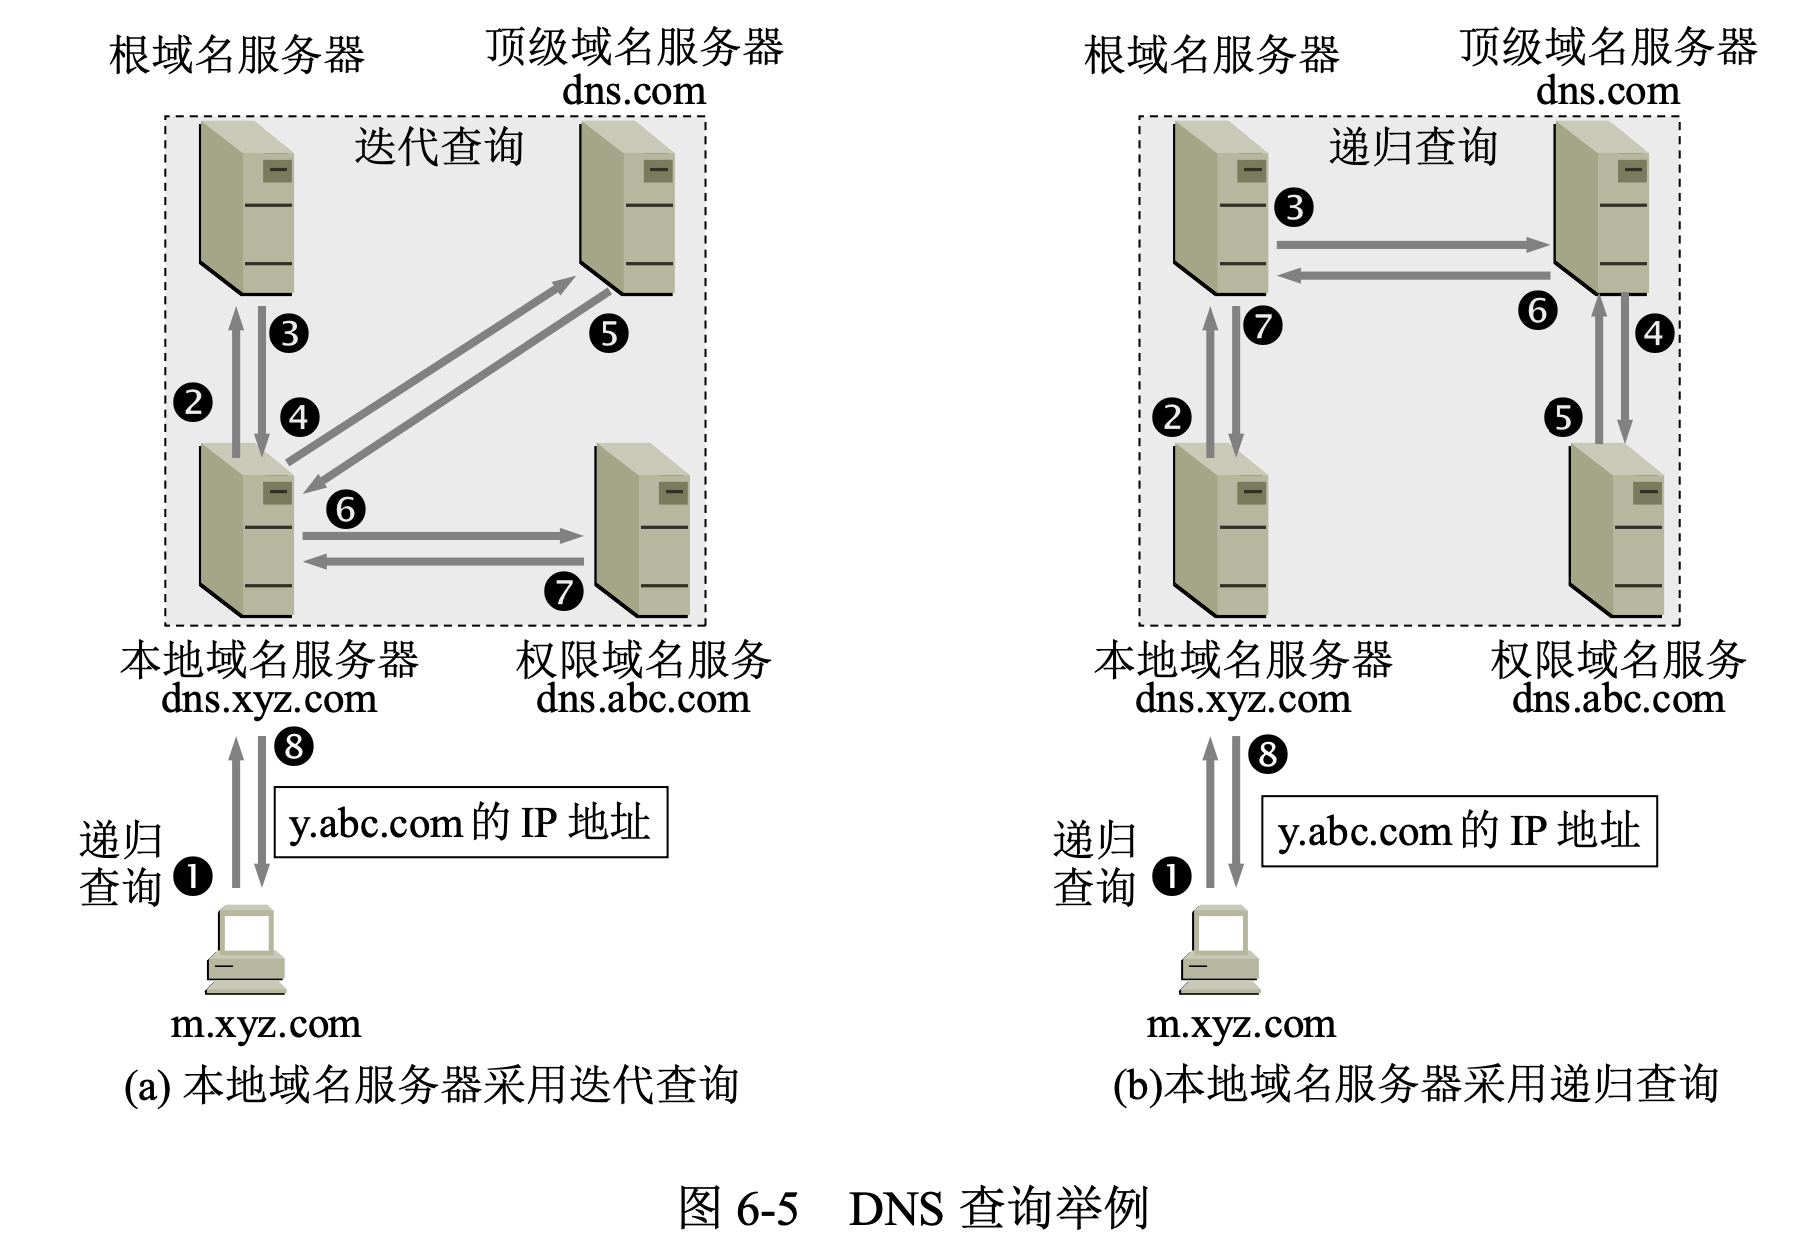
\includegraphics[width=0.8\textwidth]{img/6.5}
	\end{figure}

	\section{文件传送协议}

	\subsection{FTP概述}

	\begin{itemize}
		\item 将某台计算机中的文件通过网络传送到可能相距很远的另一台计算机中,是一项基本的网络应用,即文件传输
		\item 文件传输协议 FTP(file transfer protocol)是因特网上使用最广泛的文件传送协议
		\begin{itemize}
			\item FTP 提供交互式的访问,允许客户指明文件的类型与格式(如指明是否使用 ASCII 码),并允许文件具有存取权限(如访问文件的用户必须经过授权,并输入有效的口令)
			\item FTP 屏蔽了各计算机系统的细节,因而适合于在异构网络中任意计算机之间传送文件
		\end{itemize}
		\item 在互联网发展的早期阶段,用 FTP 传送文件约占整个互联网的通信量的三分之一,而由电子邮件和域名系统所产生的通信量还小于 FTP 所产生的通信量。只是到了 1995 年, WWW 的通信量才首次超过了 FTP
		\item 基于 TCP 的 FTP 和基于 UDP 的简单文件传送协议 TFTP,都是复制整个文件,其特点是:若要存取一个文件,就必须先获得一个本地的文件副本。如果要修改文件,只能对文件的副本进行修改,然后再将修改后的文件副本传回到原节点
		\item 文件共享协议中的另一大类是联机访问,意味着允许多个程序同时对一个文件进行存取,由操作系统提供对远地共享文件进行访问的服务。属于文件共享协议的有网络文件系统 NFS
	\end{itemize}

	\subsection{FTP的基本工作原理}
	\begin{figure}[H]
		\centering
		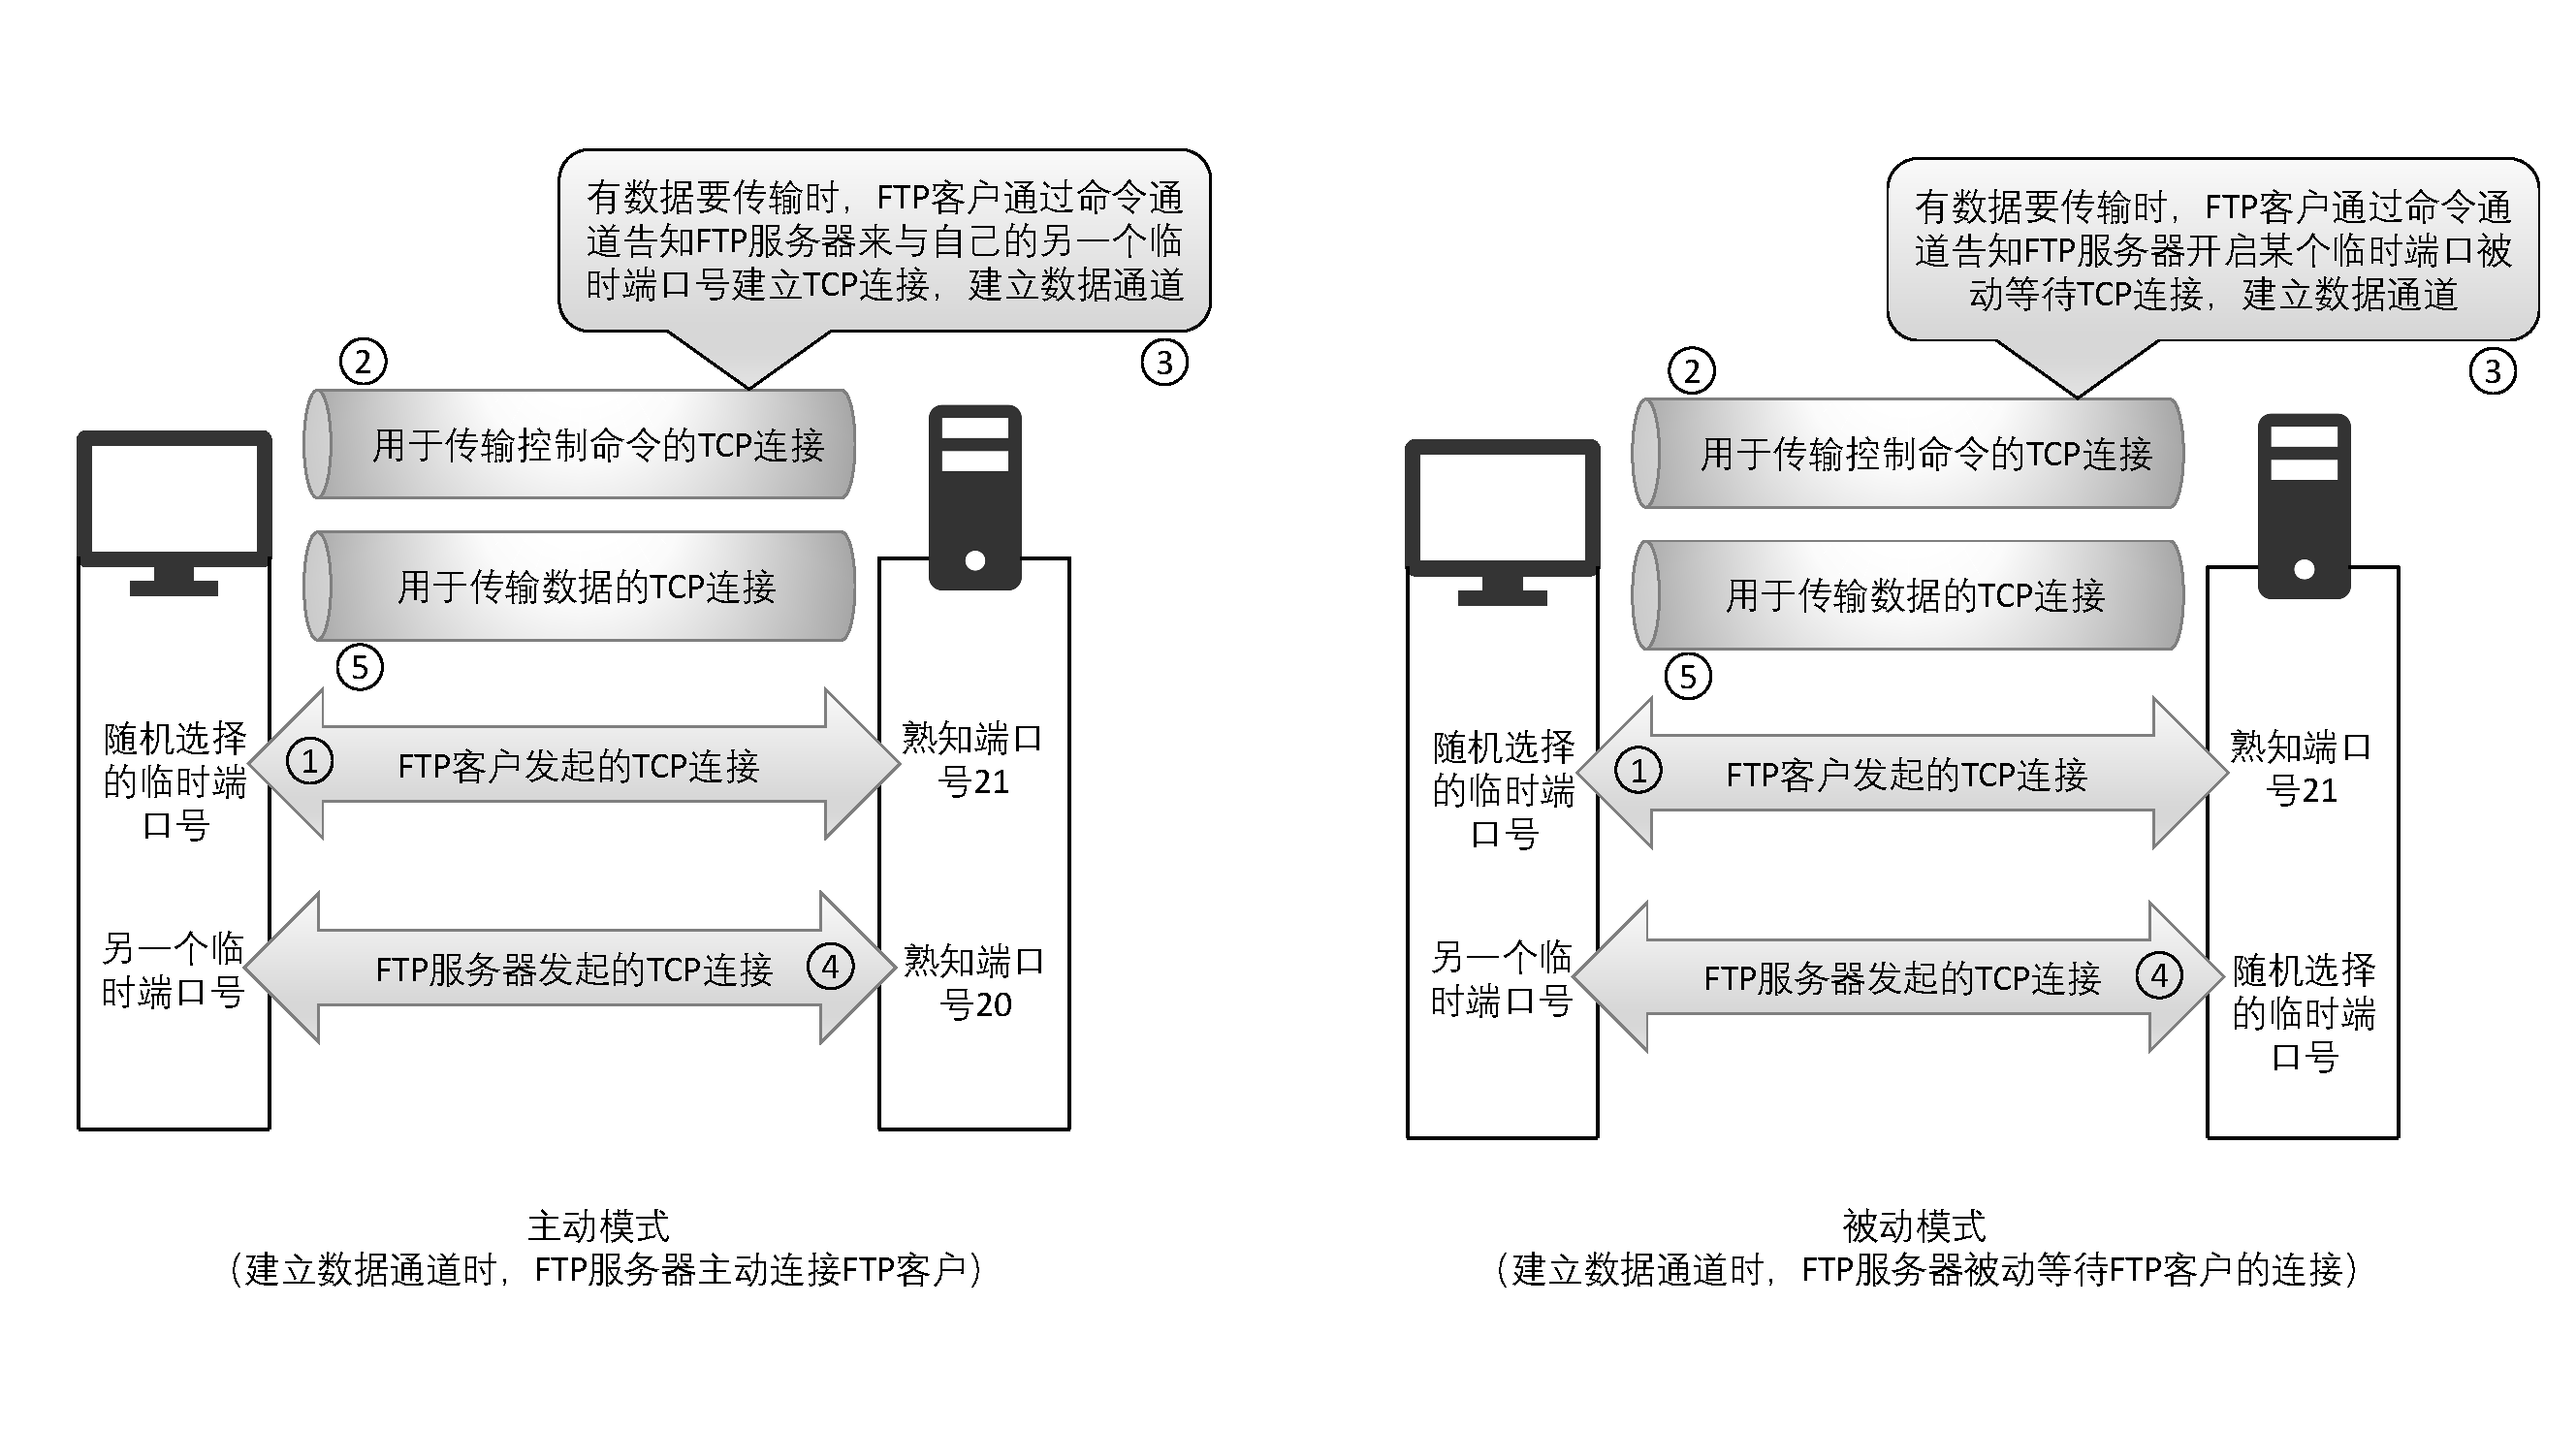
\includegraphics[width=0.9\textwidth]{img/6.2.2}
	\end{figure}

	\subsection{简单文件传送协议TFTP}
	TFTP 的主要特点是:
	\begin{itemize}
		\item 每次传送的数据报文中有 512 字节的数据,但最后一次可不足 512 字节
		\item 数据报文按序编号,从 1 开始
		\item 支持 ASCII 码或二进制传送
		\item 可对文件进行读或写
		\item 使用很简单的首部
	\end{itemize}

	TFTP 的工作很像停止等待协议
	\begin{itemize}
		\item 发送完一个文件块后就等待对方的确认,确认时应指明所确认的块编号
		\item 发完数据后在规定时间内收不到确认就要重发数据 PDU
		\item 发送确认 PDU 的一方若在规定时间内收不到下一个文件块,也要重发确认 PDU
		\item 这样就可保证文件的传送不致因某一个数据报的丢失而失败
	\end{itemize}

	在一开始工作时。TFTP 客户进程发送一个读请求报文或写请求报文给 TFTP 服务器进程,其熟知端口号码为 69。TFTP 服务器进程要选择一个新的端口和 TFTP 客户进程进行通信

	若文件长度恰好为 512 字节的整数倍,则在文件传送完毕后,还必须在最后发送一个只含首部而无数据的数据报文。若文件长度不是 512 字节的整数倍,则最后传送数据报文中的数据字段一定不满 512 字节,这正好可作为文件结束的标志

	\section{远程终端协议TELNET}

	TELNET 又称为终端仿真协议,是一个简单的远程终端协议

	用户用 TELNET 就可在其所在地通过 TCP 连接注册(即登录)到远地的另一台主机上(使用主机名或 IP 地址)。TELNET 能将用户的击键传到远地主机,同时也能将远地主机的输出通过 TCP 连接返回到用户屏幕。这种服务是透明的,因为用户感觉到好像键盘和显示器是直接连在远地主机上

	为了适应不同计算机和操作系统的差异,TELNET 定义了数据和命令应怎样通过互联网。这些定义就是所谓的网络虚拟终端 NVT 

	\begin{figure}[H]
		\centering
		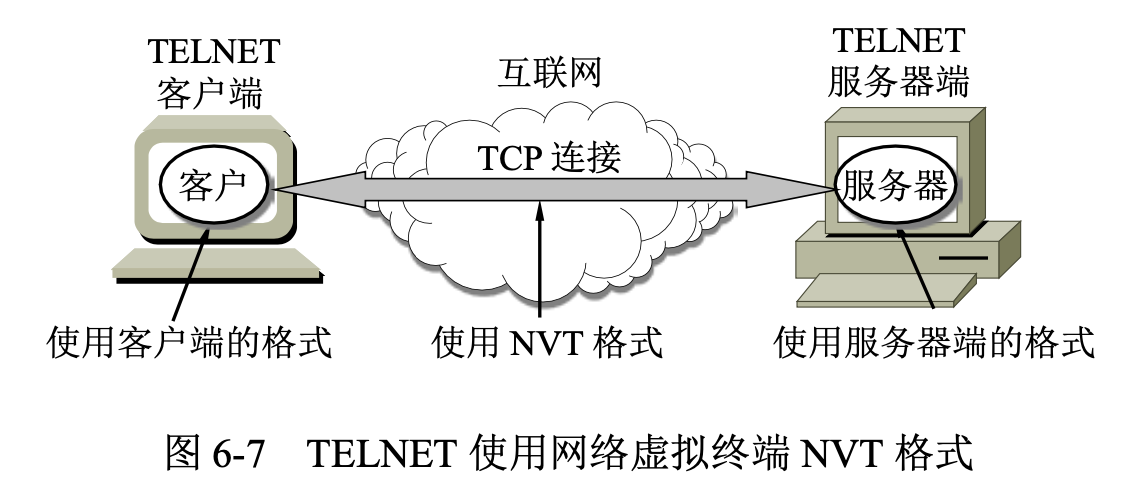
\includegraphics[width=0.6\textwidth]{img/6.7}
	\end{figure}

	\begin{itemize}
		\item 客户软件把用户的击键和命令转换成 NVT 格式,并送交服务器。服务器软件把收到的数据和命令从 NVT 格式转换成远地系统所需的格式
		\item 向用户返回数据时,服务器把远地系统的格式转换为 NVT 格式,本地客户再从 NVT 格式转换到本地系统所需的格式
		\item NVT 的格式定义很简单,所有的通信都使用 8 位一个字节
		\begin{itemize}
			\item 在运转时,NVT 使用 7 位 ASCII 码传送数据,而当高位置 1 时用作控制命令
			\item ASCII 码共有 95 个可打印字符和 33 个控制字符。所有可打印字符在 NVT 中的意义和在 ASCII 码中一样
			\item 但 NVT 只使用了 ASCII 码的控制字符中的几个
			\item 此外,NVT 还定义了两字符的 CR-LF 为标准的行结束控制符
		\end{itemize}
	\end{itemize}

	\section{万维网WWW}

	\subsection{万维网概述}

	万维网WWW(world wide web)是一个大规模的、 联机式的信息储藏所。万维网用链接的方法能非常方便地从互联网上的一个站点访问另一个站点,从而主动地按需获取丰富的信息。

	\begin{figure}[H]
		\centering
		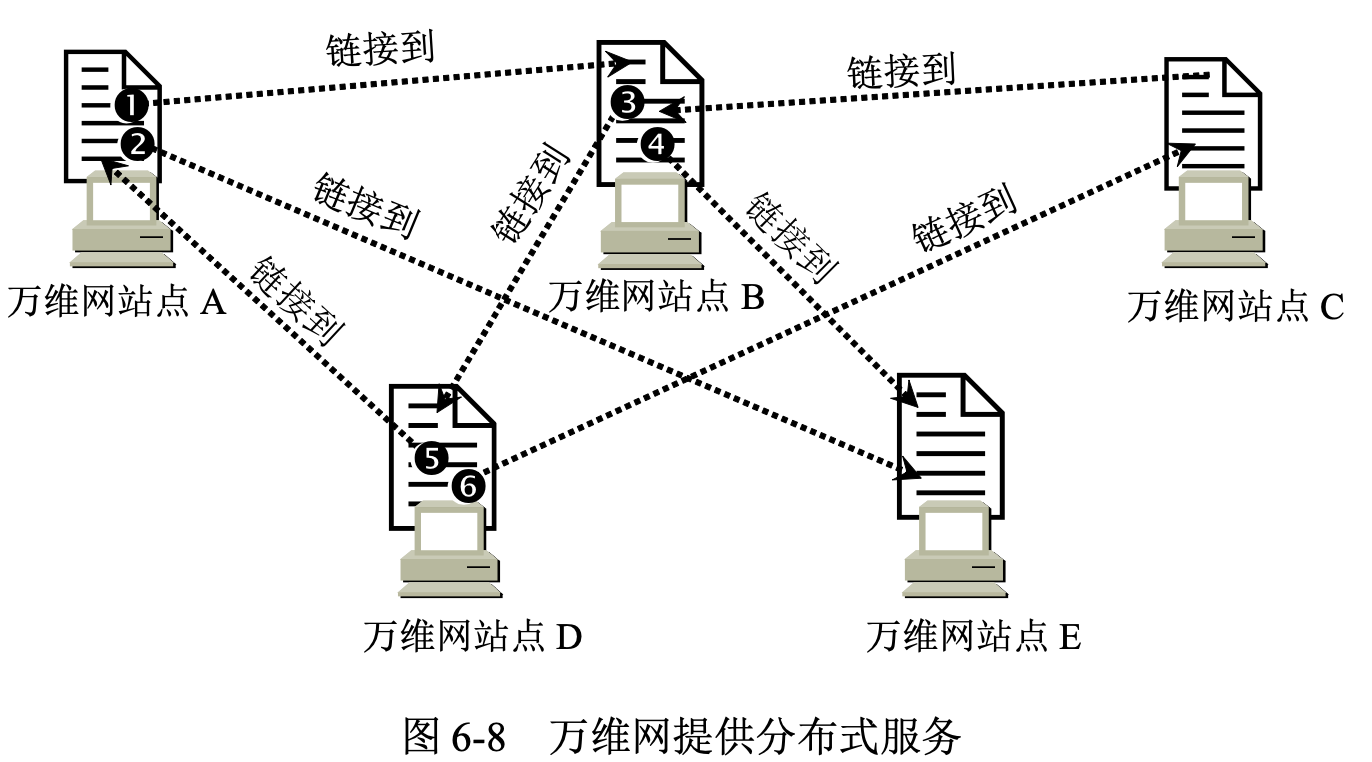
\includegraphics[width=0.7\textwidth]{img/6.8}
	\end{figure}

	万维网是一个分布式的超媒体(hypermedia)系统,它是超文本(hypertext)系统的扩充
	\begin{itemize}
		\item 超文本是指包含指向其他文档的链接的文本,一个超文本由多个信息源链接成,而这些信息源可以分布在世界各地,并且数目也是不受限制的
		\item 超媒体与超文本的区别是文档内容不同。超文本文档仅包含文本信息,而超媒体文档还包含其他表示方式的信息,如图形、图像、声音、动画以及视频图像等
	\end{itemize}

	万维网需要解决的问题及解决方式
	\begin{itemize}
		\item 怎样标志分布在整个互联网上的万维网文档:使用统一资源定位符 URL(Uniform Resource Locator)来标志万维网上的各种文档,并使每一个文档在整个互联网的范围内具有唯一的标识符 URL
		\item 用什么样的协议来实现万维网上的各种链接:万维网客户程序与万维网服务器程序之间的交互遵守超文本传送协议 HTTP(HyperText Transfer Protocol)
		\item 怎样使不同作者创作的不同风格的万维网文档,都能在互联网上的各种主机上显示出来,同时使用户清楚地知道在什么地方存在着链接:万维网使用超文本标记语言 HTML(HyperText Markup Language),使得万维网页面的设计者可以很方便地用链接从本页面的某处链接到互联网上的任何一个万维网页面,并且能够在自己的主机屏幕上将这些页面显示出来
		\item 怎样使用户能够很方便地找到所需的信息:用户可使用搜索工具在万维网上方便地查找所需的信息
	\end{itemize}

	\subsection{统一资源定位符URL}

	\subsubsection{URL的格式}
	URL 的一般形式由以下四个部分组成:
	\begin{center}
		<协议>://<主机>:<端口>/<路径>
	\end{center}

	\begin{itemize}
		\item <协议>就是指出使用什么协议来获取该万维网文档
		\item 第二部分<主机>指出这个万维网文档是在哪一台主机上,这里的<主机>就是指该主机在互联网上的域名
		\item 再后面是第三和第四部分<端口>和<路径>,有时可省略
	\end{itemize}

	\subsubsection{使用HTTP的URL}
	对于万维网的网点的访问要使用 HTTP 协议。HTTP 的 URL 的一般形式是:
	\begin{center}
		http://<主机>:<端口>/<路径>
	\end{center}

	HTTP 的默认端口号是 80,通常可省略。若再省略文件的<路径>项,则 URL 就指到互联网上的某个主页(home page),主页可以是以下几种情况之一:
	\begin{itemize}
		\item 一个 WWW 服务器的最高级别的页面
		\item 某一个组织或部门的一个定制的页面或目录。从这样的页面可链接到互联网上的与本组织或部门有关的其他站点
		\item 由某一个人自己设计的描述他本人情况的 WWW 页面
	\end{itemize}

	URL 里面的字母不分大小写,但为了便于阅读,有时故意使用一些大写字母

	\subsection{超文本传送协议HTTP}

	\subsubsection{HTTP的操作过程}

	\begin{itemize}
		\item HTTP 协议定义了浏览器(即万维网客户进程)怎样向万维网服务器请求万维网文档,以及服务器怎样把文档传送给浏览器
		\item 从层次的角度看,HTTP 是面向事务的(transaction- oriented)应用层协议,它是万维网上能够可靠地交换文件的重要基础
	\end{itemize}

	\begin{figure}[H]
		\centering
		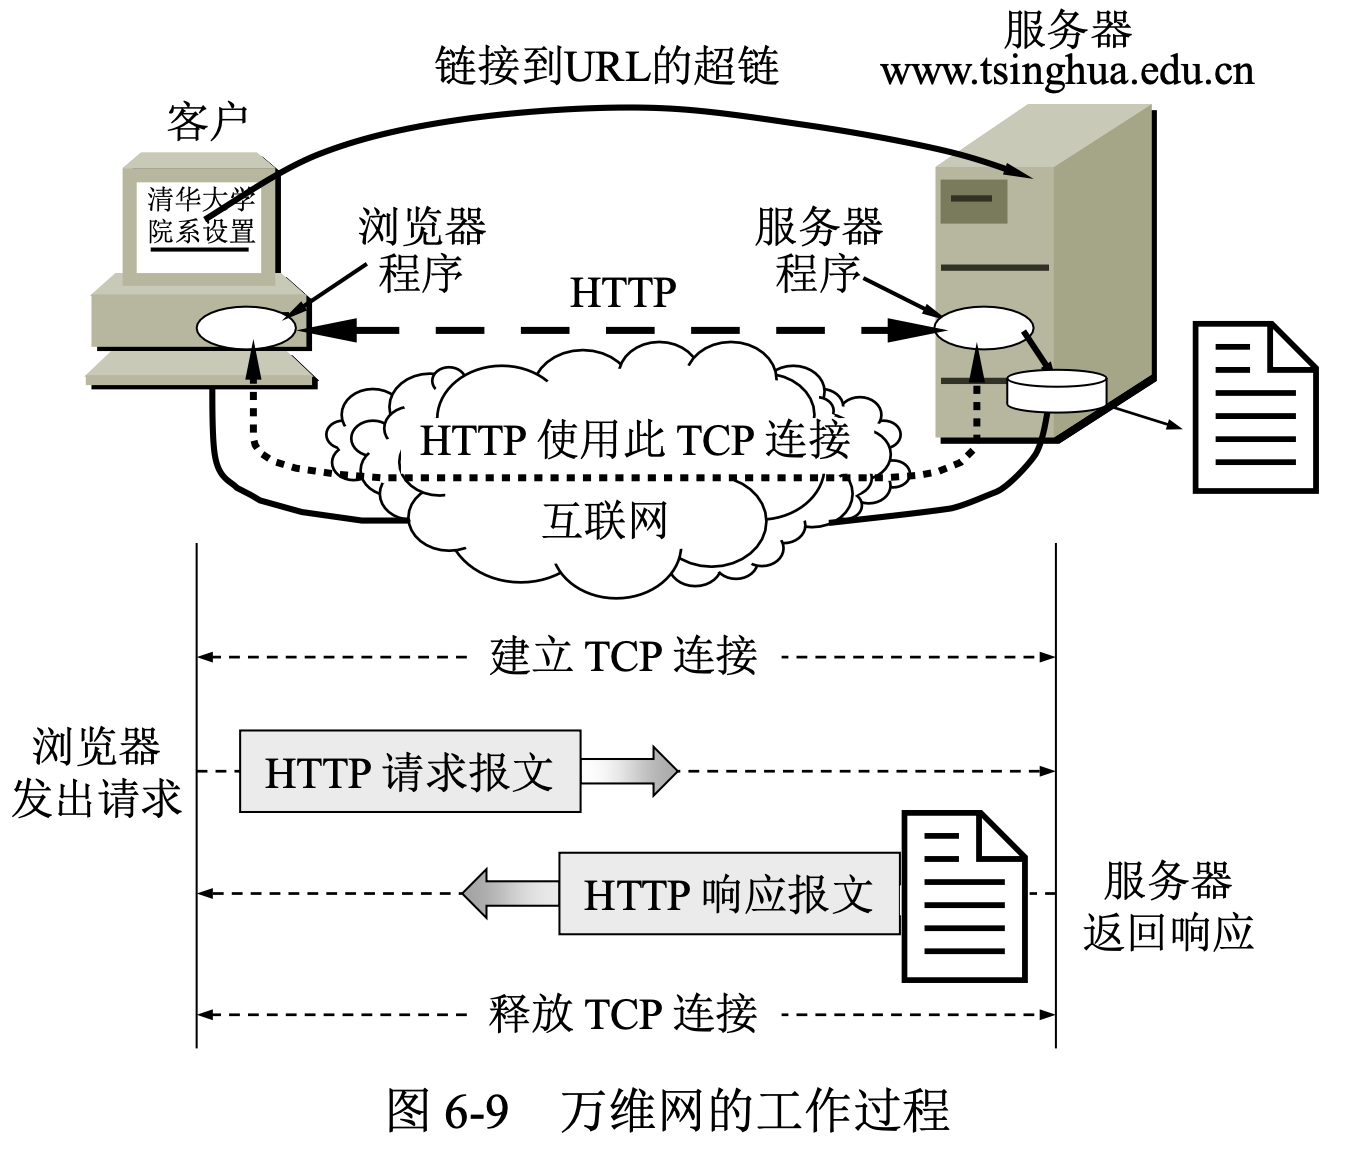
\includegraphics[width=0.65\textwidth]{img/6.9}
	\end{figure}

	\begin{itemize}
		\item HTTP 使用了面向连接的 TCP 作为运输层协议,保证了数据的可靠传输。HTTP 不必考虑数据在传输过程中被丢弃后又怎样被重传。但是,HTTP 协议本身是无连接的。这就是说,虽然 HTTP 使用了 TCP 连接,但通信的双方在交换 HTTP 报文之前不需要先建立 HTTP连接
		\item HTTP 协议是无状态的。也就是说,同一个客户第二次访问同一个服务器上的页面时,服务器的响应与第一次被访问时的相同
		\item HTTP/1.0 采用非持续连接方式。在该方式下,每次浏览器要请求一个文件都要与服务器建立 TCP 连接,当收到相应后就立即关闭连接
		\begin{itemize}
			\item 每请求一个文档就要有两倍的 RTT 的开销,若一个网页上有很多引用对象,那么请求每一个对象都需要花费 2RTT 的时间
			\item 为了减小时延,浏览器通常会建立多个并行的 TCP 连接同时请求多个对象。但是,这会大量占用万维网服务器的资源,特别是万维网服务器往往要同时服务于大量客户的请求,这会使其负担很重
		\end{itemize}
	\end{itemize}

	\begin{figure}[H]
		\centering
		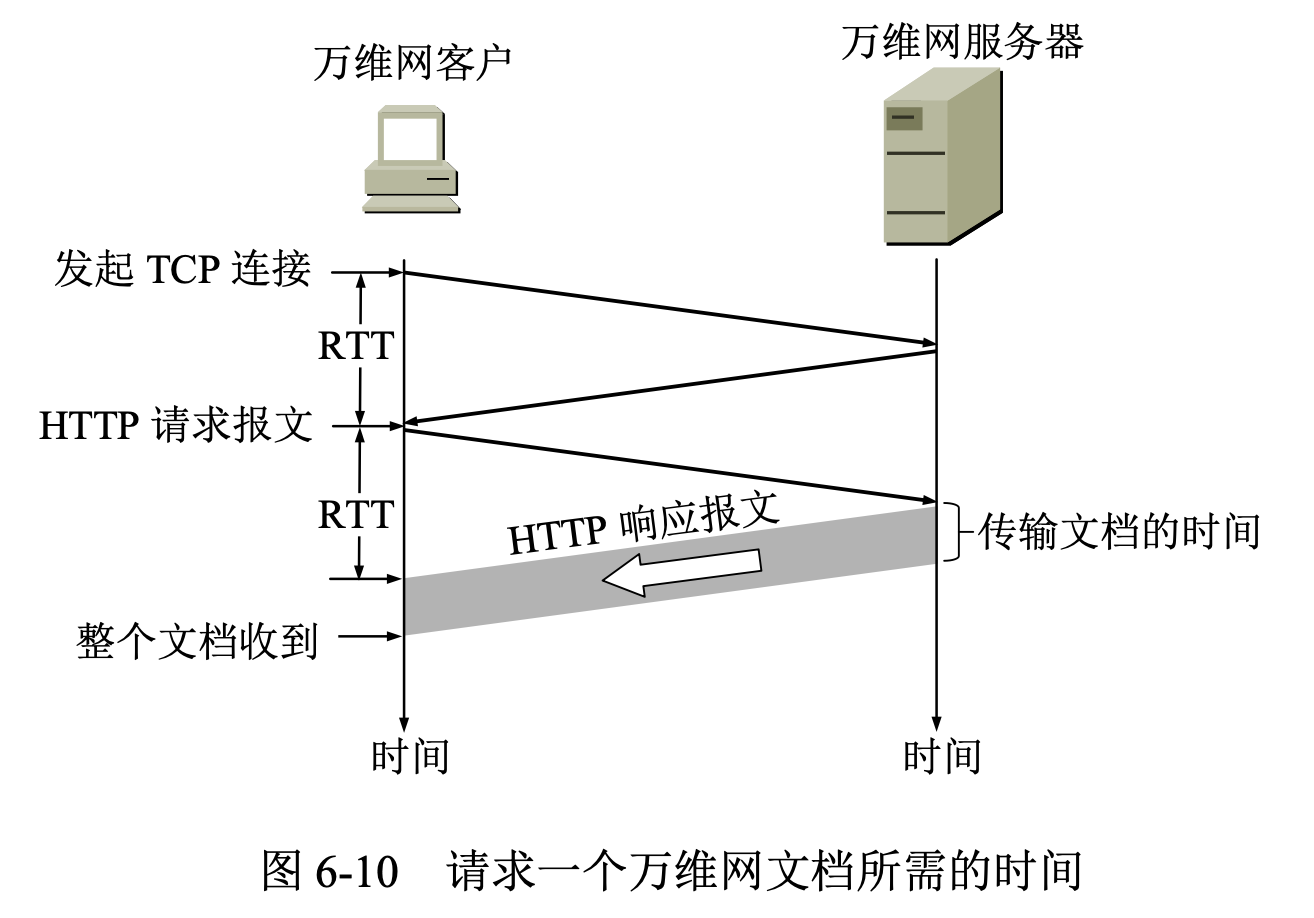
\includegraphics[width=0.55\textwidth]{img/6.10}
	\end{figure}

	\begin{itemize}
		\item HTTP/1.1 采用持续连接的方式。在该方式下,万维网服务器在发送响应后仍然保持这条连接,使同一个客户和该服务器可以继续在这条连接上传送后续的 HTTP 请求和响应报文。这并不局限于传送同一个页面上引用的对象,而是只要这些文档都在同一个服务器上就行
		\begin{itemize}
			\item 为了进一步提高效率,HTTP/1.1 的持续连接还可以使用流水线方式工作,即浏览器在收到 HTTP 的响应报文之前就能连续发送多个请求报文。这样的一个接一个的请求报文到达服务器后,服务器就发回一个接一个的响应报文。这样就节省了很多个 RTT 的时间,使 TCP 连接中的空闲时间减少,提高了下载文档的效率
		\end{itemize}
	\end{itemize}


	\subsubsection{代理服务器}
	\begin{itemize}
		\item 代理服务器(proxy server)是一种网络实体,它又称为万维网高速缓存(Web cache)
		\item 代理服务器把最近的一些请求和响应暂存在本地磁盘中
		\item 当新请求到达时,若代理服务器发现这个请求与暂时存放的请求相同,就返回暂存的响应,而不需要按 URL 的地址再次去互联网访问该资源
		\item 代理服务器可在客户端或服务器端工作,也可在中间系统上工作
	\end{itemize}

	\begin{figure}[H]
		\centering
		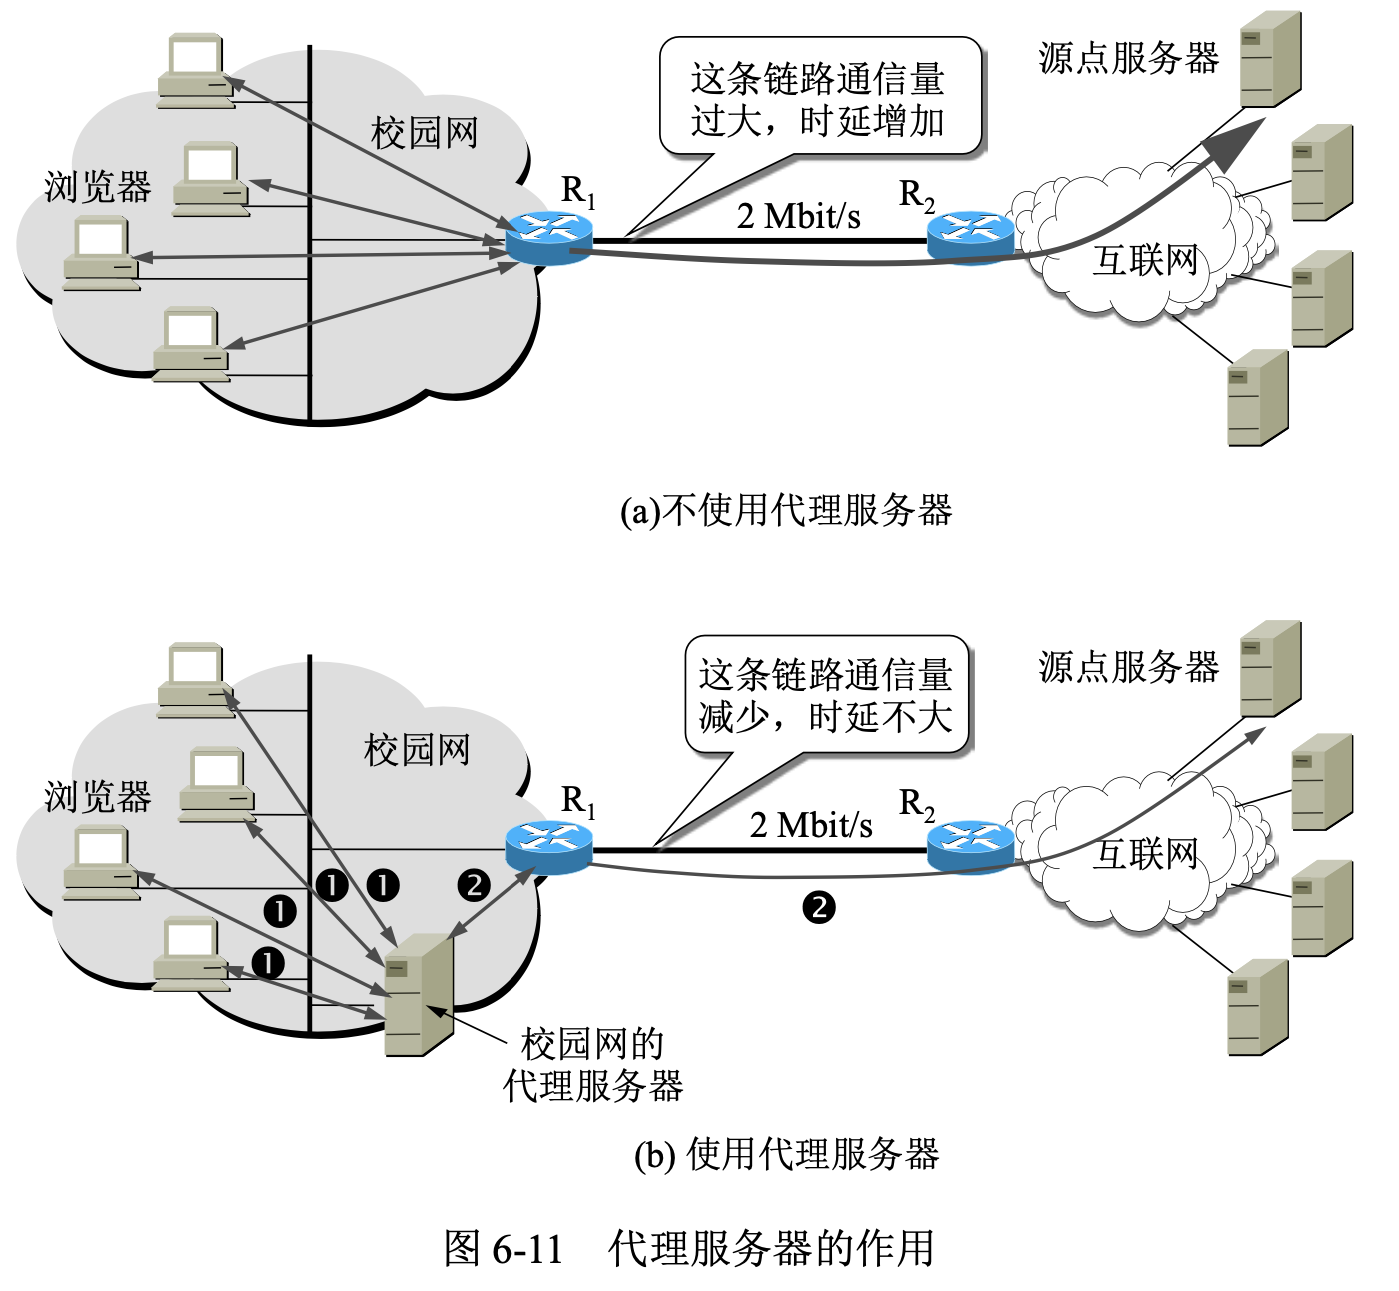
\includegraphics[width=0.5\textwidth]{img/6.11}
	\end{figure}

	\subsubsection{HTTP的报文结构}
	HTTP 有两类报文:
	\begin{itemize}
		\item 请求报文:从客户向服务器发送请求报文
		\item 响应报文:从服务器到客户的回答
	\end{itemize}

	\begin{figure}[H]
		\centering
		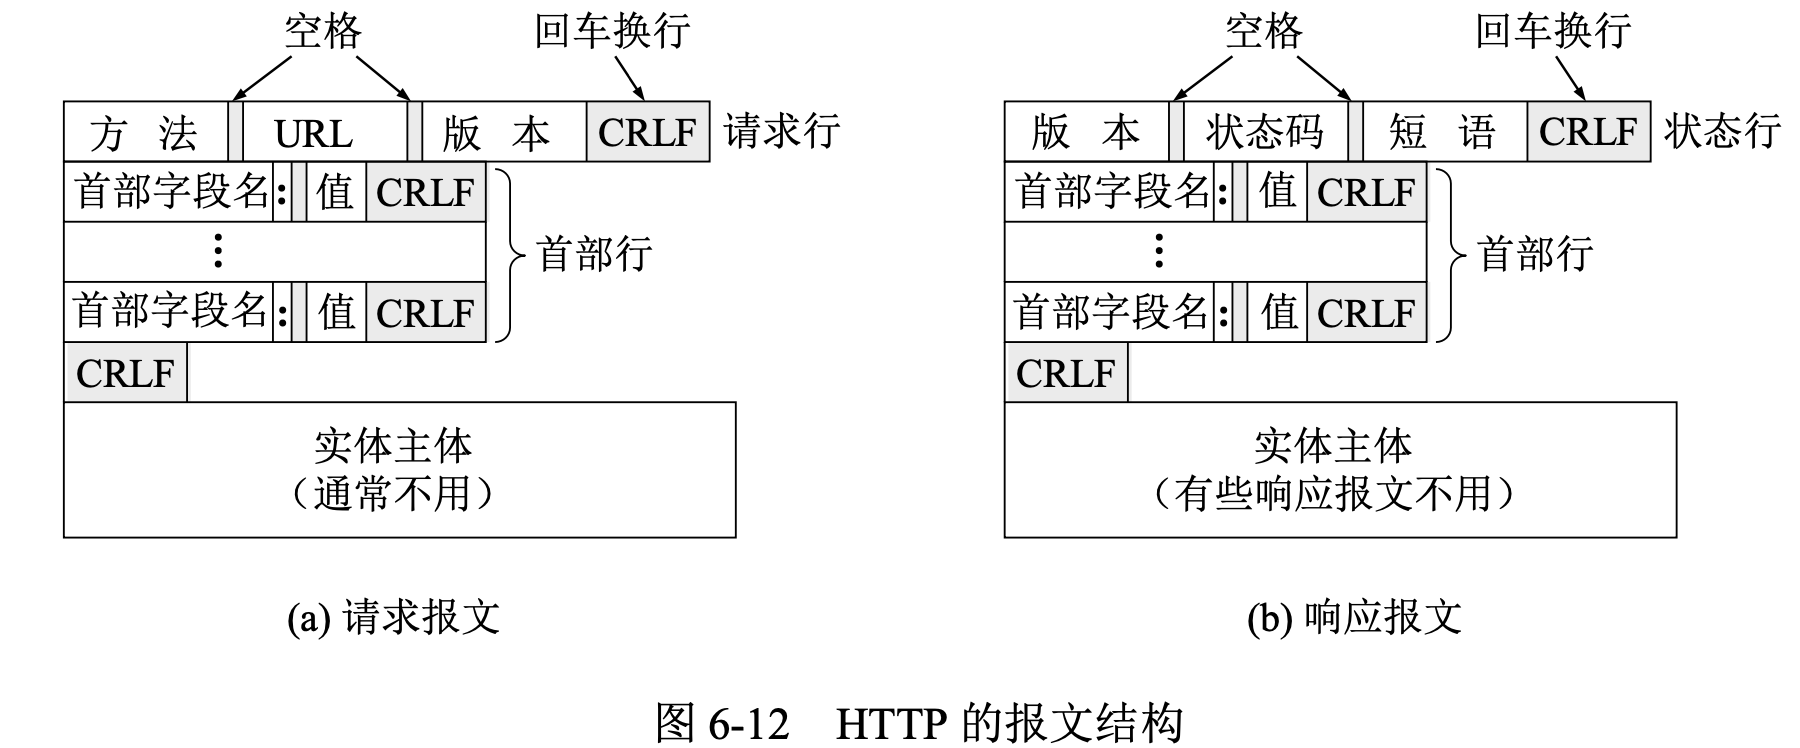
\includegraphics[width=0.7\textwidth]{img/6.12}
	\end{figure}

	由于 HTTP 是面向文本的(text-oriented),因此在报文中的每一个字段都是一些 ASCII 码串,因而各个字段的长度都是不确定的

	HTTP 请求报文和响应报文都是由三个部分组成的:
	\begin{itemize}
		\item 开始行,用于区分是请求报文还是响应报文。在请求报文中的开始行叫做请求行(Request-Line),而在响应报文中的开始行叫做状态行(Status-Line)。在开始行的三个字段之间都以空格分隔开,最后的 “CR ”和 “LF”分别代表“回车”和“换行”
		\begin{itemize}
			\item 请求报文的第一行“请求行”只有三个内容,即方法,请求资源的 URL,以及 HTTP 的版本
			\begin{itemize}
				\item “方法”是面向对象技术中使用的专门名词,对所请求的对象进行的操作,实际上也就是一些命令,请求报文中常用的几种方法如下
				\begin{table}[H]
					\centering
					\begin{tabular}{|c|c|}
					\hline
					方法(操作)  & 意义                  \\ \hline
					OPTION  & 请求一些选项的信息           \\ \hline
					GET     & 请求读取由 URL 所标志的信息    \\ \hline
					HEAD    & 请求读取由 URL 所标志的信息的首部 \\ \hline
					POST    & 给服务器添加信息(例如注释)      \\ \hline
					PUT     & 在指明的 URL 下存储一个文档    \\ \hline
					DELETE  & 删除指明的 URL 所标志的资源    \\ \hline
					TRACE   & 用来进行环回测试的请求报文       \\ \hline
					CONNECT & 用于代理服务器             \\ \hline
					\end{tabular}
				\end{table}
				\item HTTP 请求报文请求行的格式
				\begin{center}
					\verb|GET http://www.nju.edu.cn/main.htm HTTP/1.1|
				\end{center}
			\end{itemize}
			\item 响应报文的状态行包括三项内容,即 HTTP 的版本,状态码,以及解释状态码的简单短语
			\begin{itemize}
				\item 状态码都是三位数字的,分为 5 大类,这 5 大类状态码都是以不同的数字开头的
				\begin{itemize}
					\item \verb|1xx|\ 表示通知信息,如请求收到了或正在进行处理
					\item \verb|2xx|\ 表示成功,如接受或知道了
					\item \verb|3xx|\ 表示重定向,如要完成请求还必须采取进一步的行动
					\item \verb|4xx|\ 表示客户的差错,如请求中有错误的语法或不能完成
					\item \verb|5xx|\ 表示服务器的差错,如服务器失效无法完成请求
				\end{itemize}
				\item 下面三种状态行在响应报文中是经常见到的
				\begin{itemize}
					\item 接受\ \verb|HTTP/1.1 202 Accepted|
					\item 错误的请求\ \verb|HTTP/1.1 400 Bad Request|
					\item 找不到\ \verb|HTTP/1.1 404 Not Found|
				\end{itemize}
			\end{itemize}
			\item 首部行,用来说明浏览器、服务器或报文主体的一些信息。首部可以有好几行,但也可以不使用。在每一个首部行中都有首部字段名和它的值,每一行在结束的地方都要有“回车”和“换行”。整个首部行结束时,还有一空行将首部行和后面的实体主体分开
			\item 实体主体(entity body),在请求报文中一般都不用这个字段,而在响应报文中也可能没有这个字段
		\end{itemize}
	\end{itemize}

	\subsubsection{在服务器上存放用户的信息}

	\begin{itemize}
		\item 早期的万维网应用非常简单,仅仅是用户查看存放在不同服务器上的各种静态文档,因此 HTTP 被设计为一种无状态的协议,这样可以简化服务器的设计
		\item 现在,用户可以通过万维网实现各种复杂的应用,如网上购物,电子商务等,这些应用往往需要万维网服务器能够识别用户
		\item Cookie 提供了一种机制使得万维网服务器能够“记住”用户,而无需用户主动提供用户标识信息,也就是说,Cookie 是一种对无状态的 HTTP 进行状态化的技术
	\end{itemize}

	\begin{figure}[H]
		\centering
		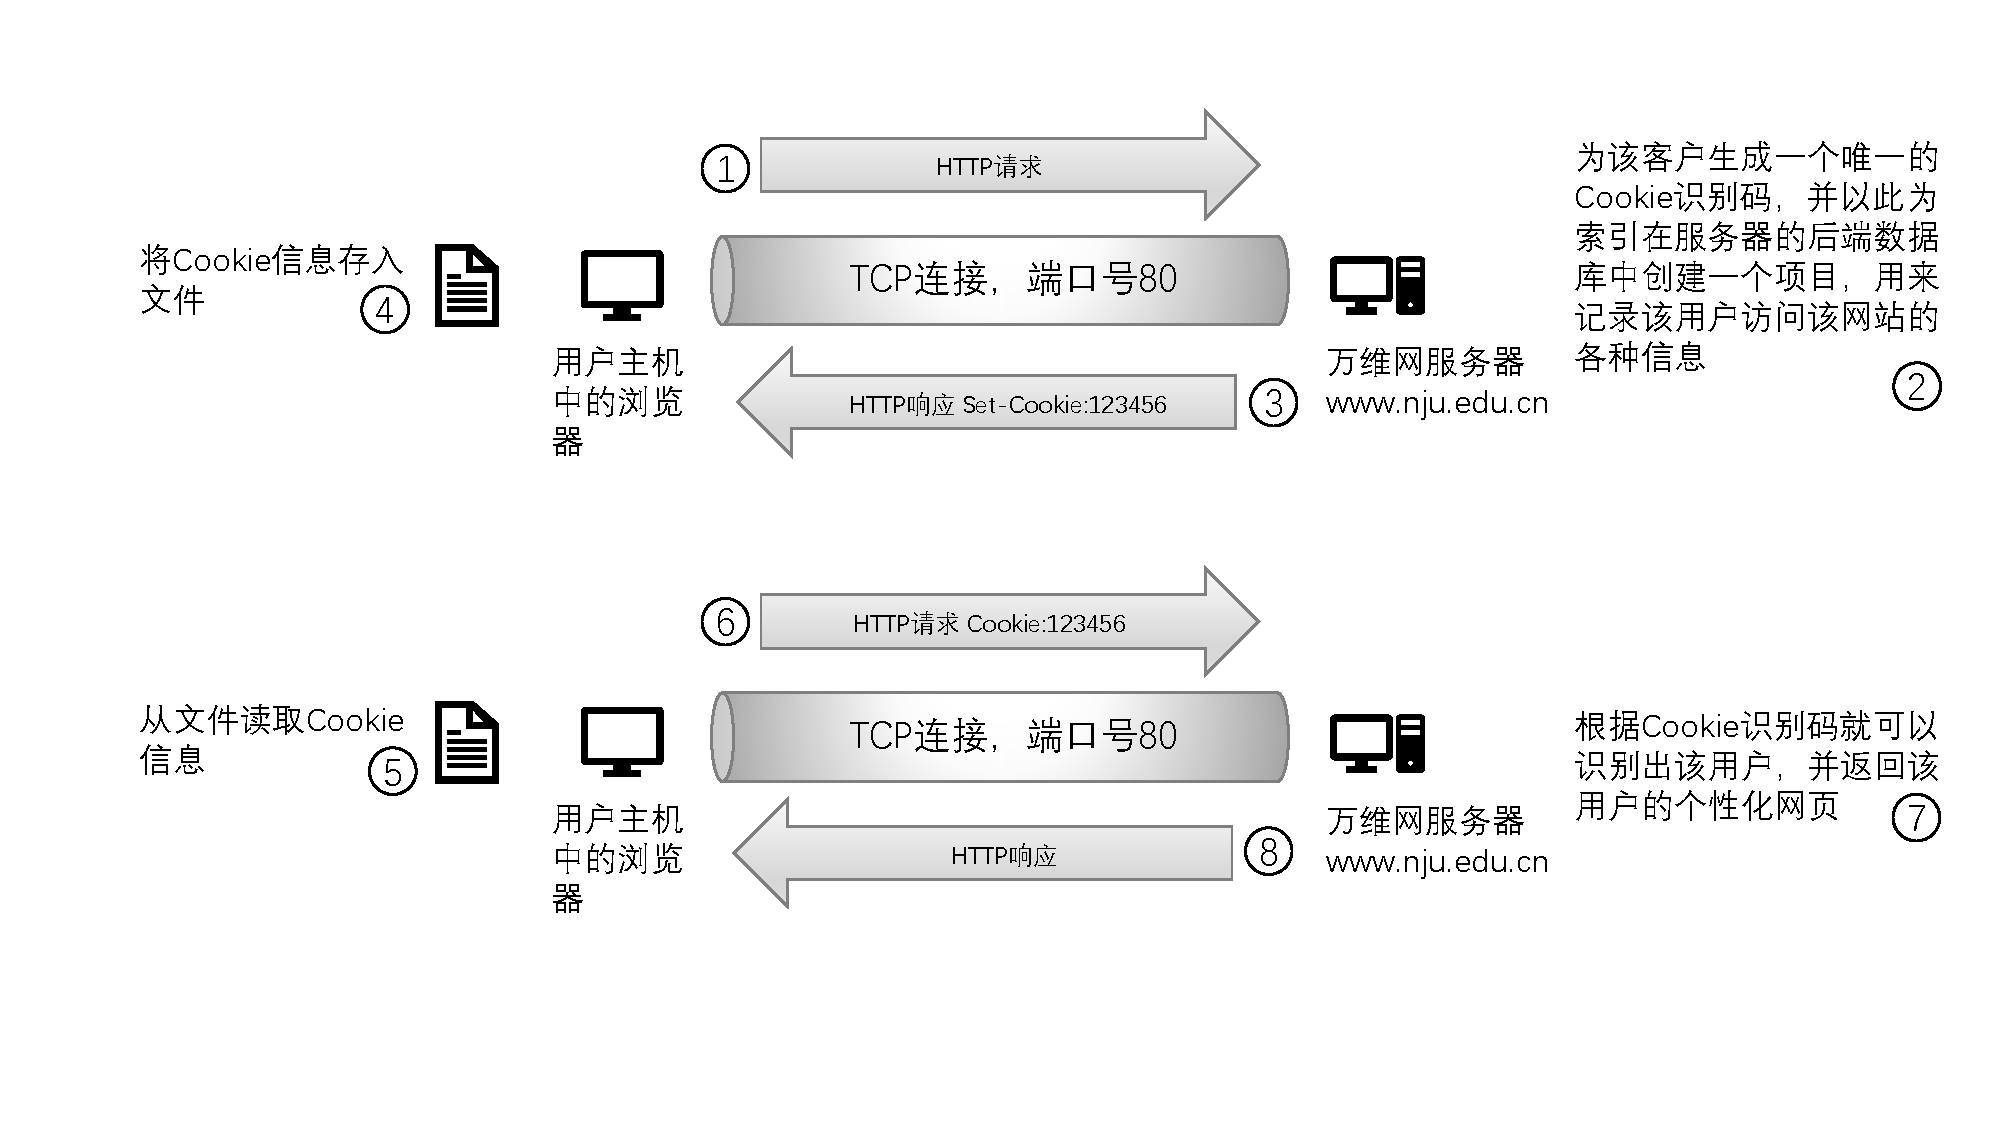
\includegraphics[width=0.8\textwidth]{img/6.4.3.4}
	\end{figure}

	\subsection{万维网的文档}

	\begin{itemize}
		\item HTML,超文本标记语言(hypertext markup language),使用多种标签来描述网页的内容和结构
		\item CSS,层叠样式表(cascading style sheet),从审美的角度来描述网页的样式
		\item JavaScript,一种脚本语言,控制网页的行为
	\end{itemize}

	\section{电子邮件}

	\subsection{电子邮件概述}
	\begin{itemize}
		\item 电子邮件是因特网上最早流行的一种应用,并且仍然是当今因特网上最重要、最实用的应用之一
		\item 传统的电话通信属于实时通信,存在以下两个缺点:
		\begin{itemize}
			\item 电话通信的主叫和被叫双方必须同时在场
			\item 一些不是十分紧迫的电话也常常没必要打断人们的工作和休息
		\end{itemize}
		\item 电子邮件与邮政系统的寄信类似
		\begin{itemize}
			\item 发件人将邮件发送到自己使用的邮件服务器
			\item 发件人的邮件服务器将收到的邮件按其目的地址转发到收件人邮件服务器中的收件人邮箱
			\item 收件人在方便的时候访问收件人邮件服务器中自己的邮箱,获取收到的电子邮件
		\end{itemize}
		\item 电子邮件使用方便、传递迅速而且费用低廉。它不仅可以传送文字信息,而且还可附上声音和图像
	\end{itemize}

	电子邮件系统的三个主要组成构件:用户代理、邮件服务器和电子邮件所需的协议
	\begin{itemize}
		\item 用户代理是用户与电子邮件系统的接口,又称为电子邮件客户端软件
		\item 邮件服务器是电子邮件系统的基础设施。因特网上所有的 ISP 都有邮件服务器,其功能是发送和接收邮件,同时还要负责维护用户的邮箱
		\item 协议包括邮件发送协议(例如 SMTP)和邮件读取协议(例如 POP3,IMAP)
	\end{itemize}

	\begin{figure}[H]
		\centering
		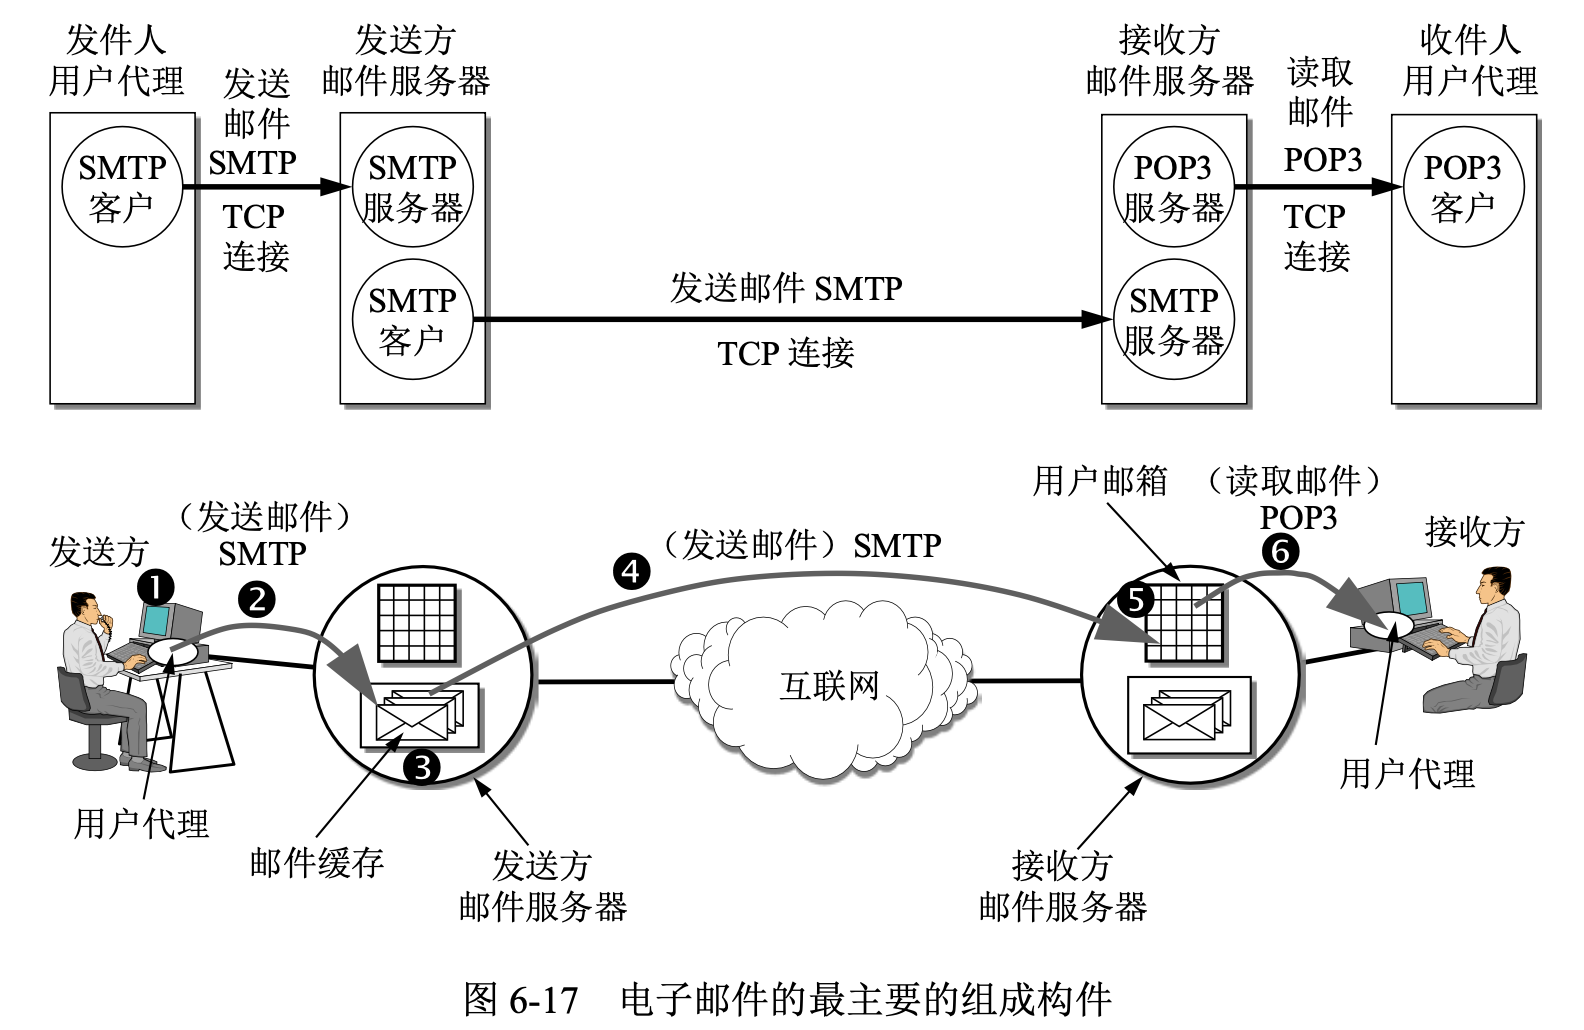
\includegraphics[width=0.8\textwidth]{img/6.17}
	\end{figure}

	\subsection{简单邮件传送协议SMTP}
	\begin{figure}[H]
		\centering
		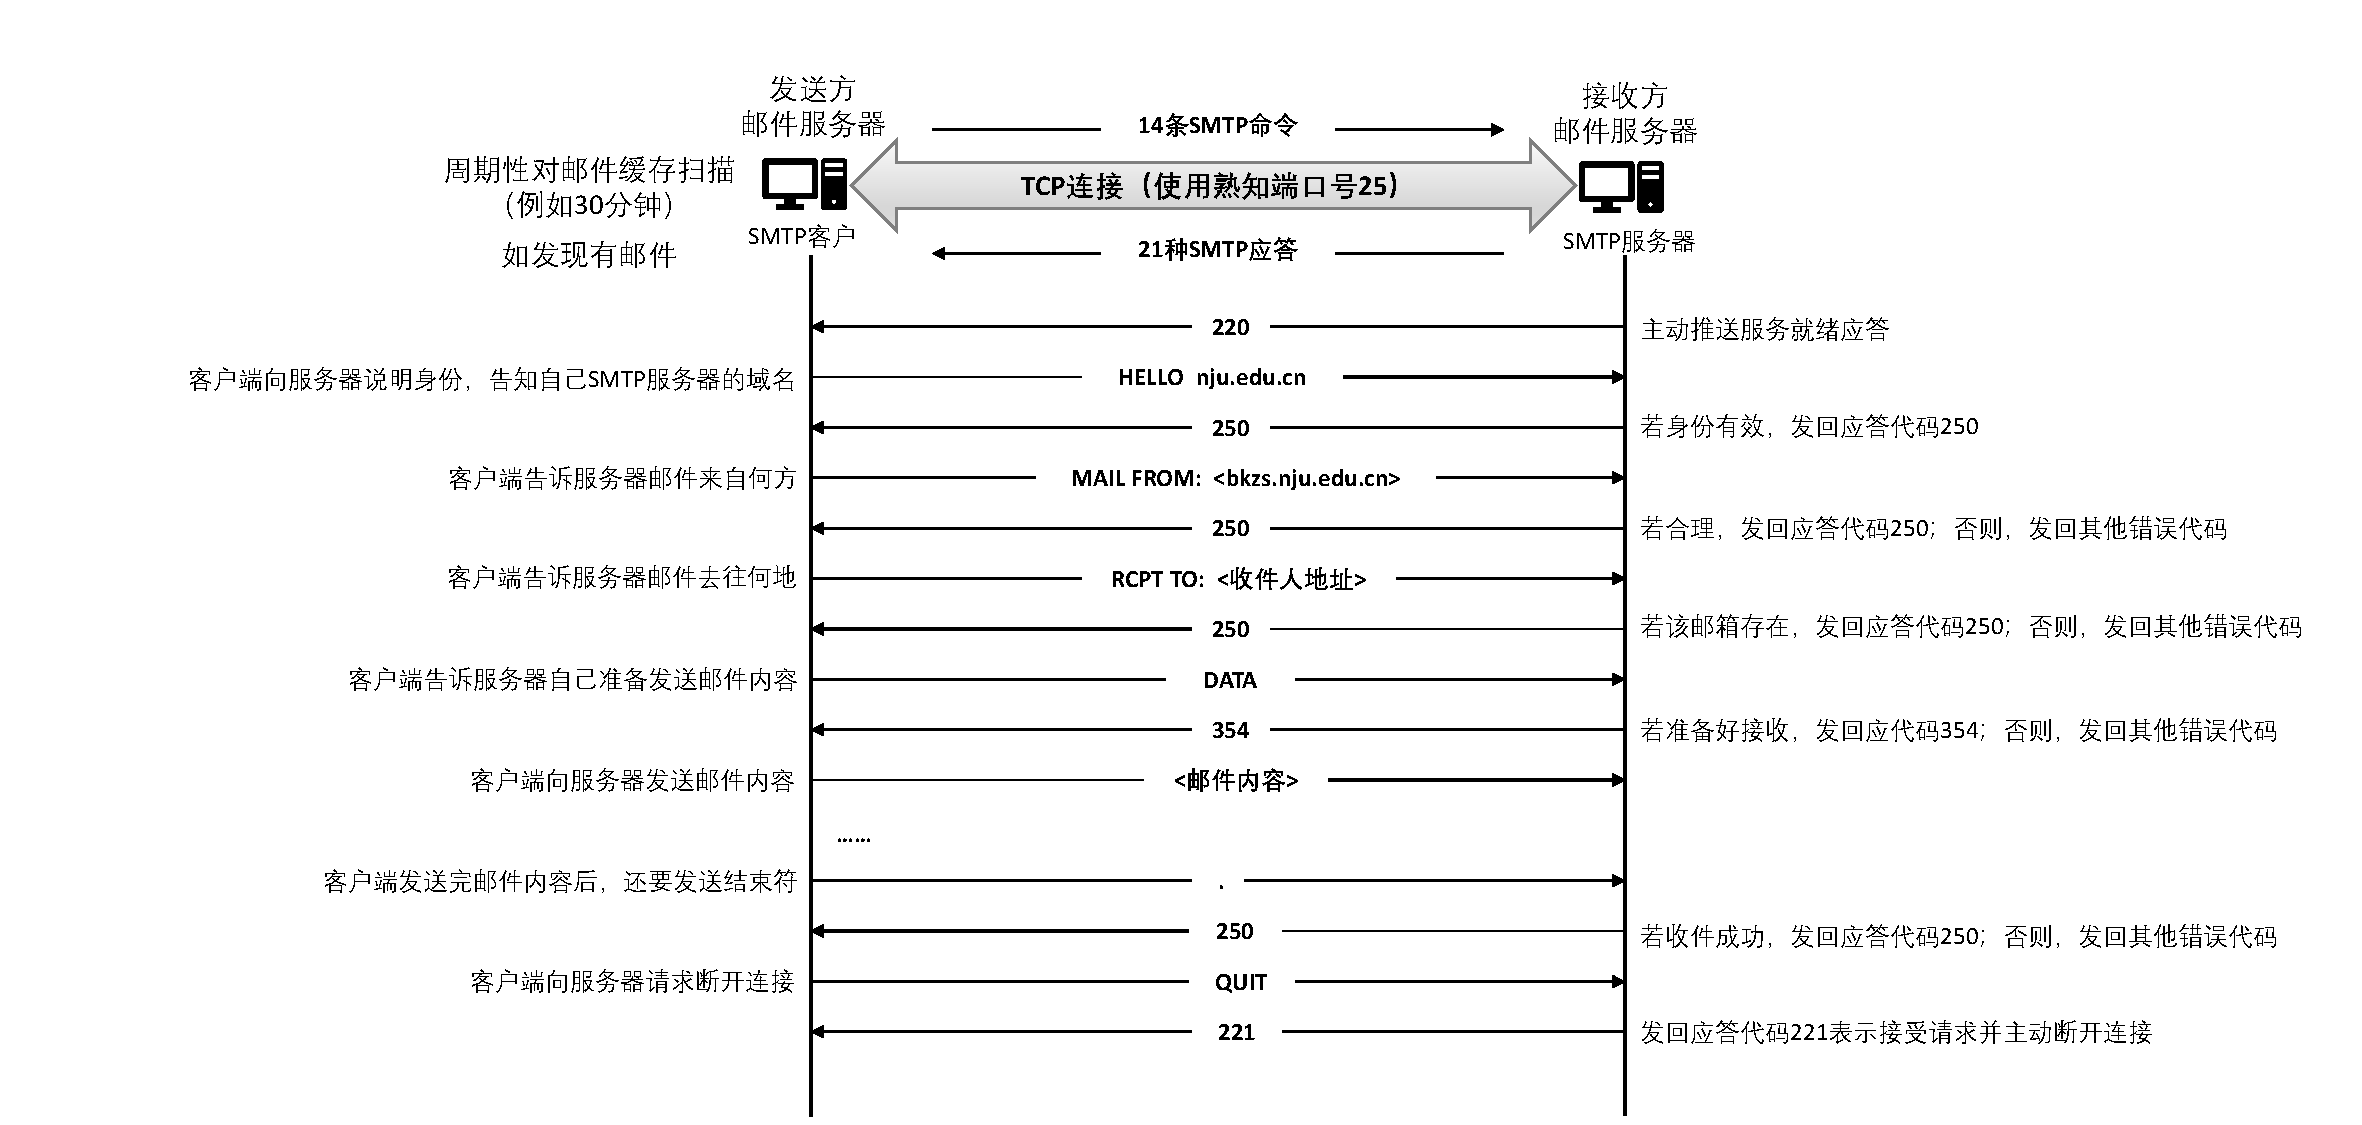
\includegraphics[width=0.98\textwidth]{img/6.5.2}
	\end{figure}

	\subsection{电子邮件的信息格式}
	一个电子邮件分为信封和内容两大部分

	在RFC 5322文档中只规定了邮件内容中的首部格式,而对邮件的主体部分则让用户自由撰写。用户写好首部后,邮件系统自动地将信封所需的信息提取出来并写在信封上。所以用户不需要填写电子邮件信封上的信息

	\subsection{邮件读取协议POP3和IMAP}
	常用的邮件读取协议有以下两个:
	\begin{itemize}
		\item 邮局协议 POP(post office protocol),POP3 是其第三个版本,是因特网正式标准
		\begin{itemize}
			\item 非常简单、功能有限的邮件读取协议。用户只能以下载并删除方式或下载并保留方式从邮件服务器下载邮件到用户方计算机。不允许用户在邮件服务器上管理自己的邮件
		\end{itemize}
		\item 因特网邮件访问协议 IMAP(Internet Message Access Protocol),IMAP4 是其第四个版本
		\begin{itemize}
			\item 功能比 POP3 强大的邮件读取协议。用户在自己的计算机上就可以操控邮件服务器中的邮箱,就像在本地操控一样,因此 IMAP 是一个联机协议
		\end{itemize}
		\item POP3 和 IMAP4 都采用基于 TCP 连接的客户/服务器方式。POP3 使用熟知端口号 110,IMAP4 使用熟知端口 143
	\end{itemize}

	\subsection{基于万维网的电子邮件}
	\begin{itemize}
		\item 通过浏览器登录邮件服务器万维网网站就可以撰写、收发、阅读和管理电子邮件。这种工作模式与 IMAP 很类似,不同的是用户计算机无需安装专门的用户代理程序,只需要使用通用的万维网浏览器
		\item 邮件服务器网站通常都提供非常强大和方便的邮件管理功能,用户可以在邮件服务器网站上管理和处理自己的邮件,而不需要将邮件下载到本地进行管理
	\end{itemize}

	\subsection{通用互联网邮件扩充MIME}

	\begin{itemize}
		\item SMTP 协议只能传送 ASCII 码文本数据,不能传送可执行文件和其他的二进制对象
		\item SMTP 不能满足传送多媒体邮件的需要,并且许多其他非英语国家的文字也无法用 SMTP 传送
		\item 为解决 SMTP 传送非 ASCII 码文本的问题,提出了多用途因特网邮件拓展 MIME(Multipurpose Internet Mail Extension)
		\begin{itemize}
			\item 增加了 5 个新的邮件首部字段,这些字段提供了有关邮件主体的信息
			\begin{itemize}
				\item MIME-Version:标志 MIME 的版本。现在的版本号是 1.0,若无此行,则为英文文本
				\item Content-Description:这是可读字符串,说明此邮件主体是否是图像、音频或视频
				\item Content-Id:邮件的唯一标识符
				\item Content-Transfer-Encoding:在传送时邮件的主体是如何编码的
				\item Content-Type:说明邮件主体的数据类型和子类型
			\end{itemize}
			\item 定义了许多邮件内容的格式,对多媒体电子邮件的表示方法进行了标准化
			\item 定义了传送编码,可对任何内容格式进行转换,而不会被邮件系统改变
		\end{itemize}
	\end{itemize}

	\begin{figure}[H]
		\centering
		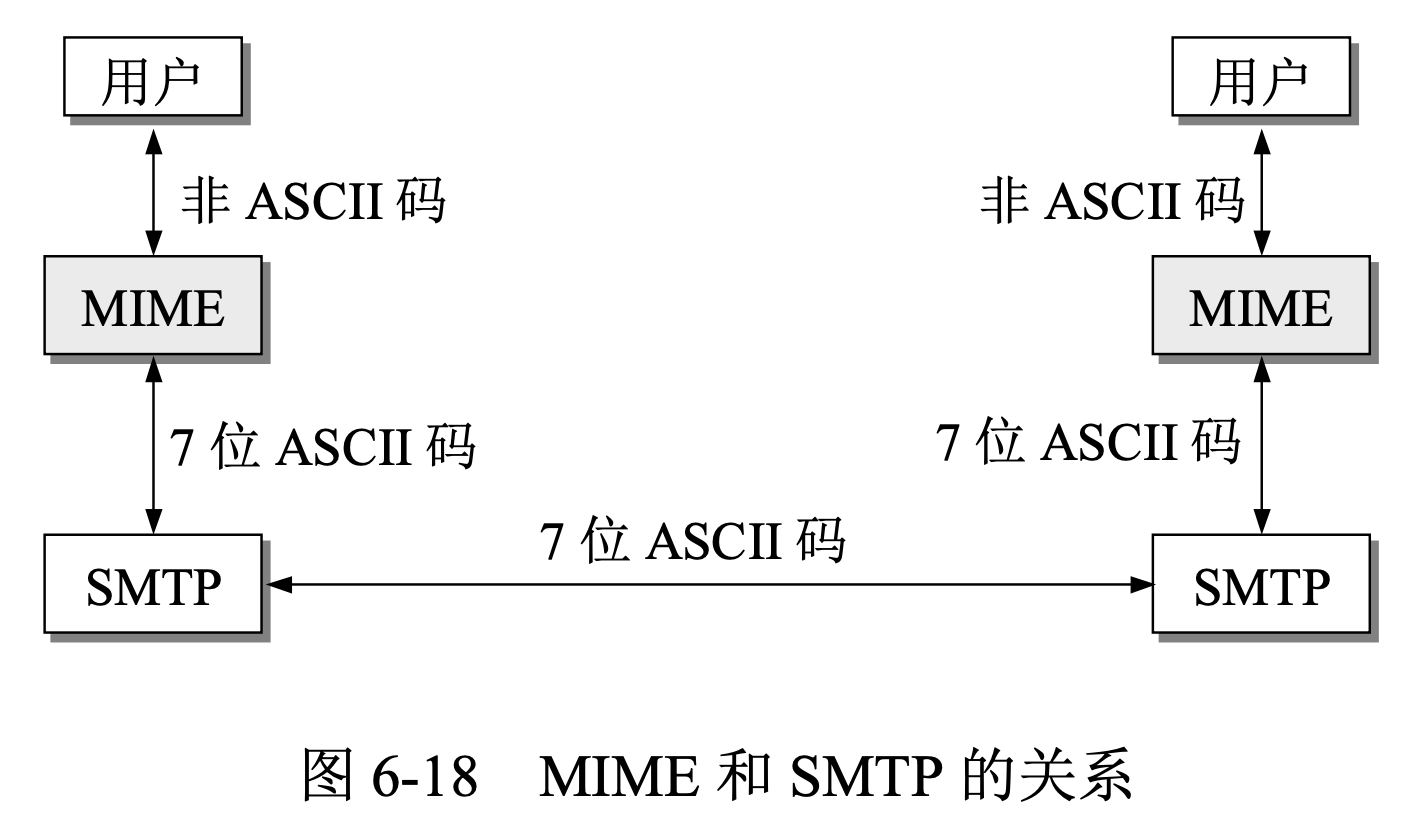
\includegraphics[width=0.5\textwidth]{img/6.18}
	\end{figure}

	\section{动态主机配置协议DHCP}

	互联网现在广泛使用的是动态主机配置协议 DHCP(Dynamic Host Configuration Protocol),它提供了一种机制,称为即插即用连网(plug-and-play networking)。这种机制允许一台计算机加入新的网络和获取 IP 地址而不用手工参与

	为了避免需要在每一个网络上都设置一个 DHCP 服务器,需要每一个网络至少有一个 DHCP 中继代理,它配置了 DHCP 服务器的 IP 地址信息。当 DHCP 中继代理收到主机 A 以广播形式发送的发现报文后,就以单播方式向 DHCP 服务器转发此报文,并等待其回答。收到 DHCP 服务器回答的提供报文后,DHCP 中继代理再把此提供报文发回给主机 A

	\begin{figure}[H]
		\centering
		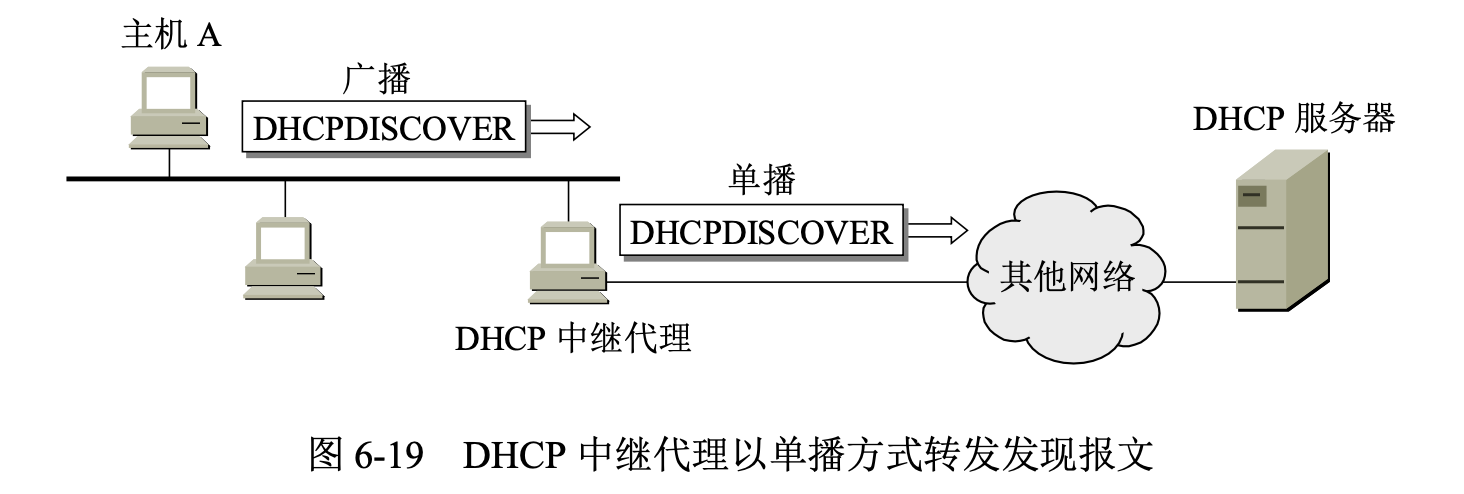
\includegraphics[width=0.6\textwidth]{img/6.19}
	\end{figure}

	下图是 DHCP 协议的工作过程
	\begin{figure}[H]
		\centering
		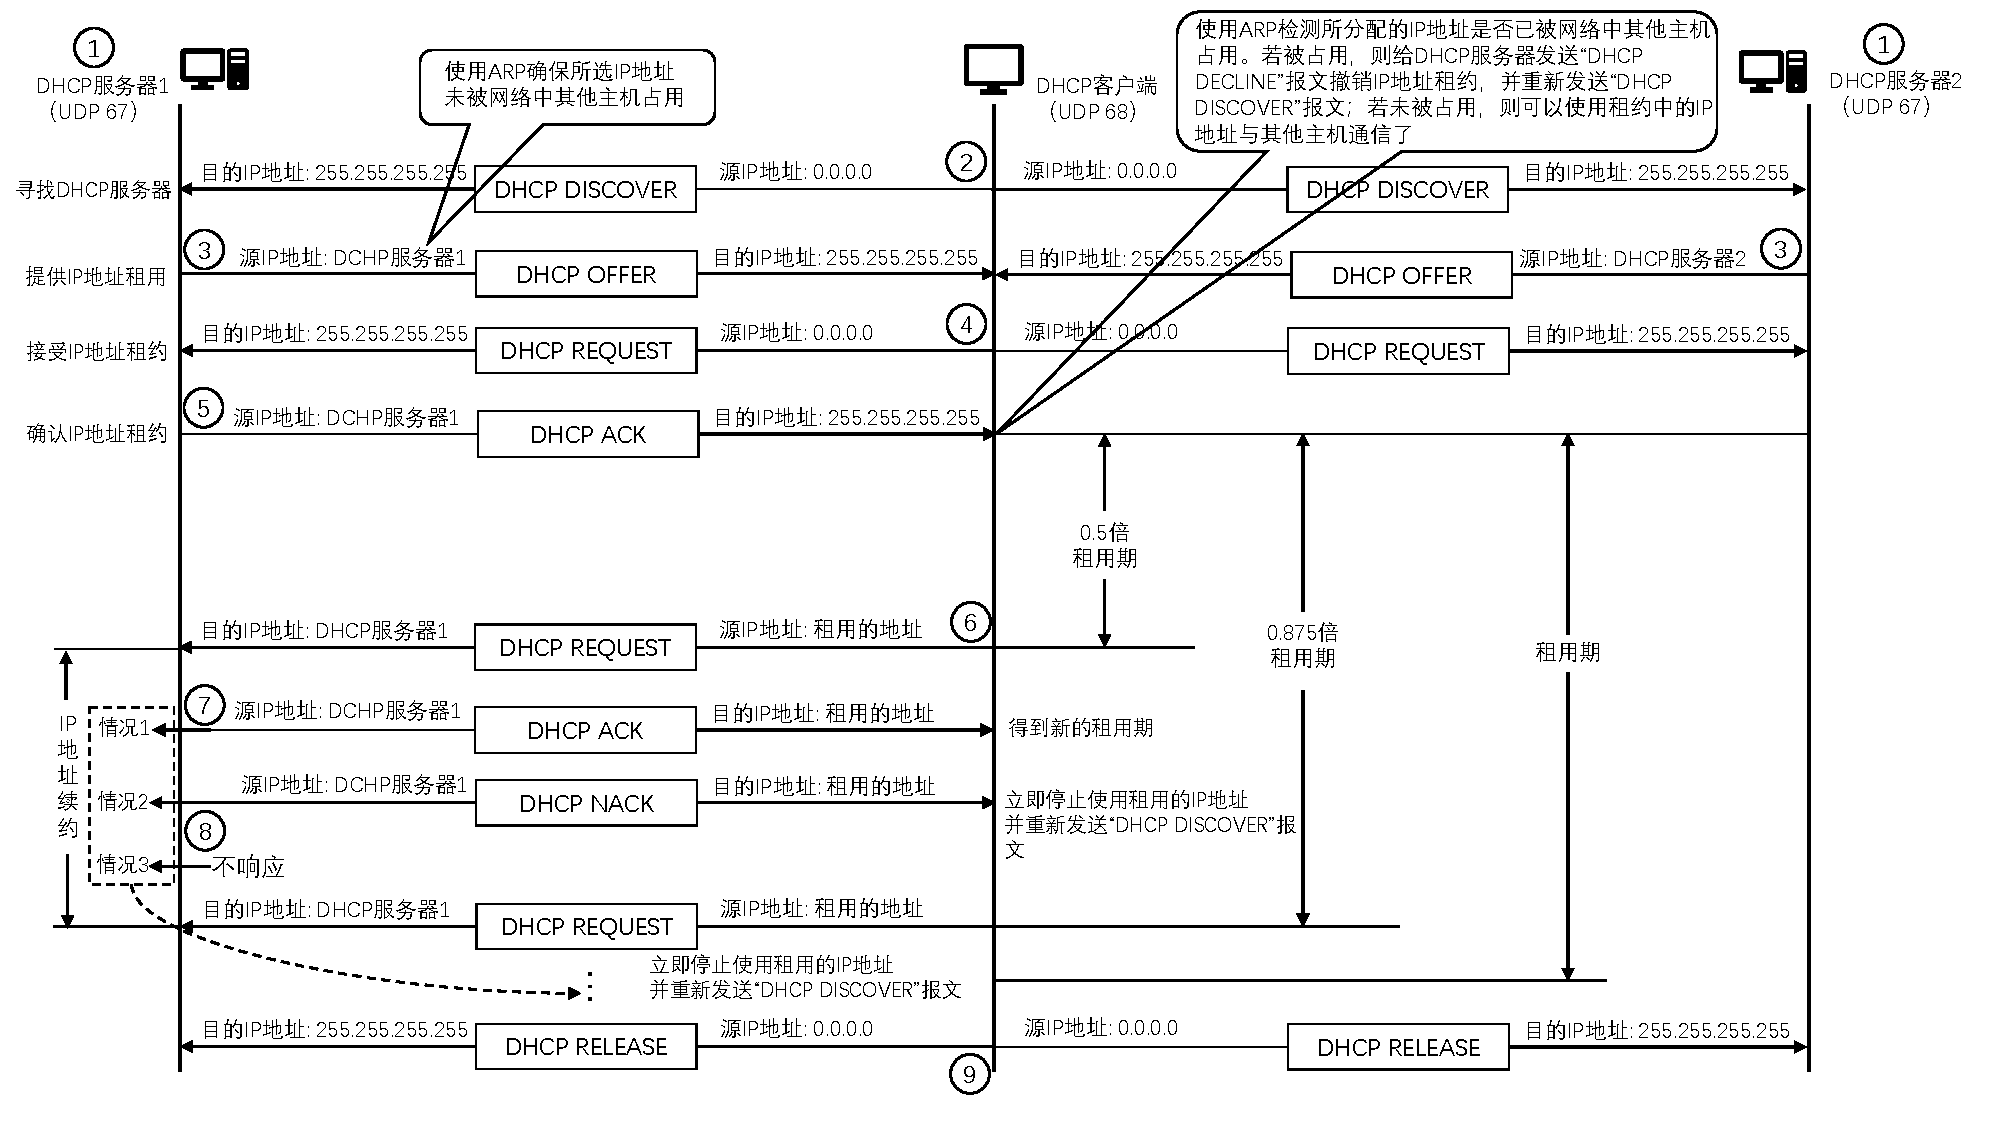
\includegraphics[width=0.98\textwidth]{img/6.6}
	\end{figure}

	\begin{enumerate}[label=\arabic*.]
		\item DHCP 服务器被动打开 UDP 端口 67,等待客户端发来的报文
		\item DHCP 客户从 UDP 端口 68 发送 DHCP 发现报文
		\item 凡收到 DHCP 发现报文的 DHCP 服务器都发出 DHCP 提供报文,因此 DHCP 客户可能收到多个 DHCP 提供报文
		\item DHCP 客户从几个 DHCP 服务器中选择其中的一个,并向所选择的 DHCP 服务器发送 DHCP 请求报文。
		\item 被选择的 DHCP 服务器发送确认报文 DHCP ACK。从这时起,DHCP 客户就可以使用这个 IP 地址了。这种状态叫做已绑定状态,因为在 DHCP 客户端的 IP 地址和硬件地址已经完成绑定,并且可以开始使用得到的临时 IP 地址了
		
		DHCP 客户现在要根据服务器提供的租用期 $T$ 设置两个计时器,它们的超时时间分别是 $0.5T$ 和 $0.875T$。当超时时间到了就要请求更新租用期
		
		\item 租用期过了一半时,DHCP 发送请求报文 DHCP REQUEST 要求更新租用期
		
		\item DHCP 服务器若同意,则发回确认报文 DHCP ACK。DHCP 客户得到了新的租用期,重新设置计时器
		
		\item DHCP 服务器若不同意,则发回否认报文 DHCP NACK。这时 DHCP 客户必须立即停止使用原来的 IP 地址,而必须重新申请 IP 地址(回到步骤 2)
		
		\item 若 DHCP 服务器不响应步骤 6 的请求报文 DHCP REQUEST,则在租用期过了 87.5\% 时,DHCP 客户必须重新发送请求报文 DHCP REQUEST(重复步骤 6),然后又继续后面的步骤。
		
		\item DHCP 客户可以随时提前终止服务器所提供的租用期,这时只需向 DHCP 服务器发送释放报文 DHCP RELEASE 即可
	\end{enumerate}

\end{document}


